\chapter{Noen sannsynlighetsfordelinger}
\label{kap:sannsynlighetsfordelinger} % Opprinnelig kapittelnr: 6

Dette kapitlet handler om sentrale diskrete sannsynlighetsfordelinger
som dukker opp i mange ulike situasjoner.
Vi legger vekt på å beskrive de forutsetninger som gir opphav til
fordelingene, samt studere de viktigste egenskapene, bl.a. forventning og
varians. Vi vil oppøve bruk av hjelpemidler for beregning av
sannsynligheter, herunder tabeller og tilnærmingsmetoder.
Spesielt viktig er tilnærmingen til normalfordelingen.
\footnote{Dette er en såkalt kontinuerlig fordeling. I Kapittel 8.4 
gis en kort omtale av egenskaper ved slike fordelinger. }

\section{Indikatorfordelingen}

La $I$ være en indikatorvariabel, dvs. $I$ kan anta verdiene $0$
eller $1$. (Se Eksempel 5.4). Lar vi $p$ betegne sannsynligheten
for at $I$ antar verdien $1$, ser sannsynlighetsfordelingen slik ut
\begin{center}
\begin{tabular}{c|cc}
   $i$    &   0    &  1 \\ \hline 
 $P(I=i)$ & $1-p $ & $p$
\end{tabular}
\end{center}
\noindent Her blir
\[E(I)=0 \cdot (1-p) + 1 \cdot p = p \]
\noindent En indikatorvariabel har spesielt den egenskapen at $I^2=I$.
Følgelig får vi
\begin{eqnarray*}
 var(I)&=&E(I^2)-{(EI)}^2=EI-{(EI)}^2 \\
       &=&EI(1-EI)=p(1-p)
\end{eqnarray*}
\noindent Indikatorvariable er i første rekke et hjelpemiddel i studiet av
andre viktige sannsynlighetsfordelinger, spesielt i forbindelse
med beregning av forventning og varians. La oss illustrere denne mulighet
med et eksempel. \\

\begin{eksempel}{Ulike øyne i terningkast}
$n$ terninger trilles. Hva blir forventet antall forskjellige
øyne som terningene viser? Definer i alt seks indikatorvariable
$I_1, I_2, \ldots, I_6$ hvor
\begin{eqnarray*}
     I_j&=&1 \mbox{\ \ hvis minst en terning viser $j$ øyne} \\
        &=&0 \mbox{\ \ hvis ingen terning viser $j$ øyne}
\end{eqnarray*}
\noindent Antall forskjellige øyne $X$ kan da skrives

\[ X=I_1+I_2+\cdots +I_6 \]

\noindent Nå blir $EI_j=P(I_j=1)=1-P(I_j=0)=1-{(5/6)}^n$ for alle $j$,
fordi sannsynligheten for at en terning ikke viser $j$ øyne er 5/6 og
de ulike terningene representerer uavhengige kast. Vi får
\begin{eqnarray*}
 EX&=&EI_1+EI_2+\cdots +EI_6 \\
   &=&6 \cdot (1-{(5/6)}^n)
\end{eqnarray*}
\noindent For $n=3$ gir dette $EX=2.53$, for $n=6$ blir $EX=3.99$, mens for
$n=12$ blir $EX=5.33$. Her ville en direkte beregning av $EX$ ved først
å finne sannsynlighetsfordelingen til $X$ bli nokså brysom.
\end{eksempel}

\section{Den binomiske fordeling}
La oss følge opp de tre forutsetningene for en binomisk
forsøksrekke fra Kapittel 4.6 :
\begin{center} \framebox[10cm]{\begin{minipage}{9cm}\rule{0cm}{0.5cm}
{\bf Binomisk situasjon :} Det utføres $n$ binomiske forsøk, dvs. 
\begin{enumerate}
\item  Hvert forsøk gir enten suksess eller fiasko.
\item  Sannsynligheten $p$ for suksess er den samme i hvert forsøk. 
\item  Forsøkene er uavhengige. 
\end{enumerate}
Antall suksesser $X$ i løpet av de $n$ forsøkene observeres. \\
  \end{minipage}} \end{center}
\noindent Vi er interessert i sannsynlighetsfordelingen til $X$. Denne
ble faktisk allerede utledet i Kapittel 4.6, og kalles {\em den binomiske
fordeling}.
\footnote{Merk at siden dette er en sannsynlighetsfordeling må
\[ 1=\sum_x p(x)=\sum_{x=0}^n \bino{n}{x}p^x{(1-p)}^{n-x} \]
\noindent som også kan bekreftes ved å anvende den såkalte
Newtons binomialformel på uttrykket ${(p+(1-p))}^n$ (se Oppgave~\ref*{kap:kombinatorikk}.29).}

\begin{center} \framebox[10cm]{\begin{minipage}{9cm}\rule{0cm}{0.5cm}
{\bf Binomisk fordeling :}  Dersom $X$ har fordelingsfunksjon
\[ p(x)=P(X=x)=\bino{n}{x}p^x{(1-p)}^{n-x} \; ; \; \; x=0,1, \ldots , n, \]
\noindent sier vi at X er {\em binomisk fordelt} med parametre ($n$,$p$).\\
  \end{minipage}} \end{center}

\noindent Vi har behov for enkle regneformler for forventning og
varians til binomiske variable. Disse er
\begin{center} \framebox[10cm]{\begin{minipage}{9cm}\rule{0cm}{0.5cm}
Dersom X er binomisk fordelt ($n$,$p$), har vi at 
\[ EX=n \cdot p \mbox{\ \ \ } varX=n \cdot p \cdot (1-p) \]
\mbox{} \vspace{-0.6\belowdisplayskip}
\end{minipage}} \end{center}

\noindent La oss prøve å begrunne formlene. Ved bruk av den vanlige
regneformelen for forventning får vi

\[ EX=\sum_x xp(x)=\sum_{x=0}^n x \bino{n}{x}p^x{(1-p)}^{n-x} \]

\noindent Dette uttrykk lar seg ikke lett forenkle, og vi forsøker derfor
en annen angrepsmåte. Definer for $j=1, 2, \ldots , n$
\begin{eqnarray*}
     I_j&=&1 \mbox{\ \ dersom j'te forsøk er suksess} \\
        &=&0 \mbox{\ \ dersom j'te forsøk er fiasko}
\end{eqnarray*}
\noindent Vi ser at vi kan skrive

\[     X=I_1+I_2+ \cdots +I_n \]

\noindent Siden forsøkene er uavhengige, blir $I_1, I_2, \ldots , I_n$
uavhengige stokastiske variable, og siden hver $I_j$ er en
indikatorvariabel, blir

\[ EI_j=P(I_j=1)=p \mbox{\ \ og \ \ } var I_j=p(1-p) \]

\noindent Ved å bruke kjent setning om forventning får vi
\begin{eqnarray*}
     EX&=&E(I_1+I_2+\cdots +I_n) \\
       &=&EI_1+EI_2+\cdots +EI_n \\
       &=&p+p+\cdots +p=np
\end{eqnarray*}
\noindent Videre blir på grunn av uavhengigheten
\begin{eqnarray*}
     varX&=&var(I_1+I_2+\cdots +I_n)\\
         &=&varI_1+varI_2+\cdots +varI_n \\
         &=&p(1-p)+p(1-p)+\cdots +p(1-p)=np(1-p)
\end{eqnarray*}
                    
\noindent Som en illustrasjon anvender vi teorien ovenfor på
 eksemplene 15, 16 og 17 i Kapittel 4.6. Disse dreide seg om henholdsvis
 myntkast, terningkast og en produksjonsprosess: \\

\noindent $X=$ antall kron i 10 myntkast er binomisk fordelt
 $(n=10,p=\frac{1}{2})$ :

\[ P(X=x)=\bino{10}{x}{(\frac{1}{2})}^x{(1-\frac{1}{2})}^{10-x} \]

\noindent Vi får $EX=n\cdot p=10 \cdot \frac{1}{2}=5$ og
 $varX=np(1-p)=10 \cdot \frac{1}{2} \cdot \frac{1}{2} = \frac{5}{2}$.\\ 

\noindent  $X=$ antall seksere i 10 terningkast er binomisk fordelt
$(n=10, p=1/6)$ :

\[ P(X=x)=\bino{10}{x}{(\frac{1}{6})}^x{(1-\frac{1}{6})}^{10-x} \]

\noindent Vi får $EX=n\cdot p=10 \cdot \frac{1}{6}=\frac{5}{3}$ og
 $varX=np(1-p)=10 \cdot \frac{1}{6} \cdot \frac{5}{6} = \frac{25}{18}$.\\ 

\noindent $X=$ antall defekte blant 100 produserte artikler er, med
defektprosent på 5, binomisk fordelt $(n=100, p=0.05)$ :

\[ P(X=x)=\bino{100}{x}{0.05}^x{(1-0.05)}^{100-x} \]

\noindent Vi får $EX=100\cdot 0.05=5$ og $var X=100\cdot 0.05\cdot
0.95=4.75$. \\

Til hjelp ved beregning av binomiske sannsynligheter er det
utarbeidet tabeller. I Appendiks~\ref{app:fordelngstabeller} 
har vi Tabell~\ref{tab:Binomisk_fordeling} som gir oss
$P(X=x)$ når $X$ er binomisk fordelt $(n,p)$ for $n$-verdier opp
til 10 og de fem $p$-verdiene $0.05, 0.1, 0.2, 0.3$ og $0.4$ samt
Tabell~\href{tab:Binomisk_fordeling_p05} for $p=0.5$ og $n$ helt opp til 30. For $p$-verdier og
$n$-verdier som ikke dekkes av disse tabellene, må vi ofte ty til
større tabellverker. Disse gir som regel de såkalte kumulative
sannsynligheter $P(X\leq x)$ istedenfor $P(X=x)$. Det finnes
slike tabeller for $n$ helt opp til 1000 og $p$-verdier i sprang på
$0.01$. For store verdier av $n$ vil vi i Kapittel 6.5 utvikle en
metode for tilnærmet beregning av $P(X\leq x)$. \\


\begin{eksempel}{Eksamen}
En eksamen består av åtte spørsmål hvor en i hvert spørsmål har
valget mellom fem svar hvorav ett er riktig. For å bestå eksamen
kreves minst tre riktige svar. Hva er sannsynligheten for at en
elev som er helt uforberedt, og som velger sine svar tilfeldig,
ikke består eksamen? Vi betrakter de åtte spørsmålene som 
åtte uavhengige forsøk, hvor sannsynligheten for suksess (dvs. riktig
svar) er $p=1/5=0.2$ i hvert forsøk. Lar vi $X$ betegne antall
riktige svar, blir $X$ binomisk fordelt $(n=8, p=0.2)$ :
                                                   
\[ P(X=x)=\bino{8}{x}{(\frac{1}{5})}^x{(1-\frac{1}{5})}^{8-x} \]

	\noindent Av Tabell~\ref{tab:Binomisk_fordeling} med $n=8$ og $p=0.2$ finner vi
\begin{center} \scriptsize \addtolength{\tabcolsep}{-0.5\tabcolsep}
\begin{tabular}{c|ccccccccc|c}
    $x$& 0 & 1 & 2 & 3 & 4 & 5 & 6 & 7 & 8 & sum \\ \hline
 $P(X=x)$&0.1678&0.3355&0.2936&0.1468&0.0459&0.0092&0.0011&0.0001&0.0000&1.0000
\end{tabular}
\end{center}
\noindent Sannsynlighetene er her gitt med fire desimalers nøyaktighet,
eksempelvis er sannsynligheten for åtte riktige svar positiv, men
så liten at det ikke syns i fjerde desimal. Vi får nå at
sannsynligheten for å stryke blir
\begin{eqnarray*}
P(X\leq 2)&=&P(X=0)+P(X=1)+P(X=2) \\
          &=&0.1678+0.3355+0.2936=0.7969
\end{eqnarray*}
Sannsynligheten for å bestå finnes enklest slik:

\[ P(X\geq 3)=1-P(X\leq 2)=1-0.7969=0.2031 \]

\noindent men kan også finnes ved å summere i tabellen.
Merk at $EX=np=8\cdot 0.2=1.6$ og $var X=np(1-p)=1.28$. Dette kan
selvsagt også (mer tungvint) finnes ved direkte beregning ut fra
tabellen ovenfor.
\end{eksempel}

\begin{eksempel}{Ti myntkast}
Lar vi $X=$ antall kron i ti myntkast, ser vi av en binomisk
tabell med $n=10$ og $p=0.5$ (Tabell~\ref{tab:Binomisk_fordeling_p05}) at
\begin{center}
\begin{tabular}{c|cccccc}
   $x$   &   0   &    1   &    2   &    3   &    4   &    5\\ \hline
$P(X=x)$& 0.0010 & 0.0098 & 0.0439 & 0.1172 & 0.2051 & 0.2461
\end{tabular}
\end{center}
\noindent Her merker vi oss at tabellen ikke direkte gir sannsynlighetene
for 6, 7, 8, 9 og 10 kron, men dette er heller ikke nødvendig.
Lar vi $X'=$ antall mynt i ti myntkast, er det klart at også $X'$
er binomisk fordelt $(n=10,p=0.5)$. Vi får derfor
\begin{eqnarray*}
     P(X=6)=&P(X'=4)=&0.2051 \\
     P(X=7)=&P(X'=3)=&0.1172 \mbox{\ \ osv.}
\end{eqnarray*}
\noindent slik at disse sannsynlighetene også er gitt ved tabellen.
\end{eksempel}

\begin{eksempel}{Levende mus}
En biolog driver forsøk med levende mus, og vet av erfaring at
gjennomsnittlig ca. 80\% av musene overlever slike eksperimenter.
Hvor mange mus må hun starte med dersom sannsynligheten skal være
minst 0.98 for at 5 eller flere mus overlever eksperimentet. Anta hun starter
med $n$ mus, hver mus representerer et forsøk med
to utfall, den overlever eller dør. Det er nå rimelig å anta at
sannsynligheten for at en mus overlever er 0.80. Videre antar vi
at død/overlever for de ulike mus er uavhengige begivenheter (en
noe mer tvilsom antakelse). Med disse antakelsene blir 
antall mus som overlever $X$ binomisk fordelt $(n,p=0.8)$. Vi skal
altså bestemme $n$ slik at

\[ P(X\geq 5)\geq 0.98 \]

\noindent Vi trenger derfor $P(X=x)$ for $p=0.8$ og ulike $n$. Nå ser vi at
Tabell~\ref{tab:Binomisk_fordeling} ikke dekker tilfellet $p=0.8$. Vi skal imidlertid greie
oss likevel : Betrakt isteden $X'=$ antall mus som dør. Siden
$X'=n-X$, kan vi skrive\\ $P(X=x)=P(X'=n-x)$. Vi ser at $X'=n-X$
blir binomisk fordelt $(n, p=0.2)$, og følgelig kan vi likevel
finne $P(X=x)$ ved hjelp av denne tabellen. La oss forsøke om det
er nok å starte med syv mus. Med $n=7$ og $p=0.2$ finner vi av
Tabell~\ref{tab:Binomisk_fordeling}

\begin{center}  \small \addtolength{\tabcolsep}{-0.4\tabcolsep}
\begin{tabular}{c|ccccccccc}
   $x$  &  0   &   1  &  2   &   3  &   4  &  5   &  6   & 7 \\ \hline
$P(X=x)$&0.0000&0.0004&0.0043&0.0287&0.1147&0.2753&0.3670&0.2097
\end{tabular}
\end{center}

\noindent Vi ser at $P(X\geq 5)=0.2753+0.3670+0.2097=0.8520$. Syv mus er
altså for lite. På tilsvarende måte finner vi at med $n=8$ blir
$P(X\geq 5)=0.9437$ som også er for lite. La oss derfor prøve
$n=9$. Vi finner av Tabell~\ref{tab:Binomisk_fordeling} følgende sannsynligheter :

\begin{center}\scriptsize \addtolength{\tabcolsep}{-0.5\tabcolsep}
\begin{tabular}{c|cccccccccc}
   $x$  &  0   &   1  &  2   &   3  &   4  &  5   &  6   & 7 & 8 & 9\\ \hline
$P(X=x)$&0.0000&0.0000&0.0003&0.0028&0.0165&0.0661&0.1762&0.3020&0.3020&0.1342
\end{tabular}
\end{center}

\noindent Her blir $P(X\geq 5)=0.9805$, dvs. ni mus er tilstrekkelig.
\end{eksempel}

\section{Den hypergeometriske fordeling}

Betrakt følgende problemstilling :
\begin{center} \framebox[10cm]{\begin{minipage}{9cm}\rule{0cm}{0.5cm}
 {\bf Den hypergeometriske situasjon :} \\
Gitt en populasjon bestående av $N$ objekter hvorav
\begin{center}
\begin{tabular}{rll}
            $M$ & er spesielle &(f.eks. defekte) \\
          $N-M$ & er vanlige   &(f.eks. intakte)
\end{tabular}
\end{center}
\noindent Fra populasjonen trekkes et tilfeldig uordnet utvalg på $n$
ele\-menter og antall spesielle elementer $Y$ i utvalget noteres. \\
\end{minipage}} \end{center}

\noindent Vi ønsker å finne sannsynlighetsfordelingen til $Y$.
Ifølge forutsetningen er alle $\bino{N}{n}$ mulige utvalg like
sannsynlige. Antall gunstige utvalg for begivenheten at vi får
$y$ spesielle elementer i utvalget finnes slik: De $y$ spesielle
elementene i utvalget kan velges blant de $M$ spesielle
elementene i populasjonen på $\bino{M}{y}$ måter. For hver av
disse $\bino{M}{y}$ måtene er det $\bino{N-M}{n-y}$ ulike måter å
velge ut de $n-y$ vanlige elementene i utvalget. Følgelig er det
$\bino{M}{y}\cdot \bino{N-M}{n-y}$ gunstige utvalg for
begivenheten $(Y=y)$. Sannsynlighetsfordelingen til $Y$ er derfor
gitt i følgende definisjon :
\begin{center} \framebox[10cm]{\begin{minipage}{9cm}\rule{0cm}{0.5cm}
{\bf Hypergeometrisk fordeling :} \\
 Dersom $Y$ har fordelingsfunksjon
\noindent
\[ p(y)=P(Y=y)= \frac{\bino{M}{y} \cdot \bino{N-M}{n-y}}{\bino{N}{n}} \] 

sier vi at $Y$ er {\em hypergeometrisk fordelt} $(N,M,n)$.\\
  \end{minipage}} \end{center}
\noindent Vi har behov for enkle regneformler for forventning og varians
til hypergeometrisk fordelte variable. Disse er

\begin{center} \framebox[10cm]{\begin{minipage}{9cm}\rule{0cm}{0.5cm}
Dersom $Y$ er hypergeometrisk fordelt $(N,M,n)$, så er

\[ EY=n \cdot \frac{M}{N} \mbox{\ \ \ }
        varY=\frac{N-n}{N-1} \cdot n \cdot \frac{M}{N} \cdot (1-\frac{M}{N}) \]
\mbox{}  \end{minipage}} \end{center}
\noindent La oss prøve å begrunne formlene. Ved bruk av den vanlige
regneformelen for forventning får vi

\[ EY=\sum_y yp(y)=\sum_y y 
                  \frac{\bino{M}{y} \cdot \bino{N-M}{n-y}}{\bino{N}{n}} \] 

\noindent men dette uttrykk lar seg ikke lett forenkle. La oss isteden
prøve en annen  angepsmåte, ved bruk av indikatorer:
Vi vet at et tilfeldig (uordnet) utvalg kan oppnås ved å trekke
et tilfeldig ordnet utvalg og så se bort fra rekkefølgen av
elementene. La oss derfor definere
\begin{eqnarray*}
     I_j&=&1 \mbox{\ \  dersom det j'te element i utvalget er spesielt} \\
        &=&0 \mbox{\ \ dersom det j'te element i utvalget er vanlig }
\end{eqnarray*}
\noindent Vi kan da skrive $Y$ som en sum av indikatorvariable

\[ Y=I_1+I_2+\cdots +I_n \]

\noindent Ifølge ekvivalensloven for et tilfeldig ordnet utvalg, har hvert
av de $N$ elementene i populasjonen samme sannsynlighet for å
komme på j'te plass i utvalget (se Kapittel 3.5). Herav følger at

\[ EI_j=P(I_j=1)=\frac{M}{N} \]
\[ varI_j=EI_j(1-EI_j)=\frac{M}{N}(1-\frac{M}{N}) \]
\noindent Ved å bruke kjent setning om forventning får vi 
\begin{eqnarray*}
     EY&=&E(I_1+I_2+\cdots +I_n) \\
       &=&EI_1+EI_2+\cdots +EI_n \\
       &=&\frac{M}{N}+\frac{M}{N}+\cdots \frac{M}{N}=n \cdot \frac{M}{N} 
\end{eqnarray*}
\noindent Når det gjelder variansen er problemet ikke så enkelt fordi
 $I_1,I_2, \ldots I_n$ ikke er uavhengige stokastiske variable, og
formelen om at variansen til en sum er lik summen av variansen
kan derfor ikke nyttes. Vi må trekke inn ko\-va\-rianser, og de som
er interessert i å følge den videre argumentasjon, finner den som  
 $\star$ -merket stoff ved slutten av avsnittet. \\

La oss belyse forholdet mellom den hypergeometriske fordeling og den
binomiske fordeling :

Dersom de $n$ trekningene isteden skjer med tilbakelegging, er det
klart at vi har en binomisk situasjon: Hver trekning gir enten et
spesielt eller vanlig objekt, sannsynligheten for et spesielt
objekt er $M/N$ i hver trekning og trekningene er uavhengige. I
dette tilfellet blir $Y$ binomisk fordelt $(n, p=M/N)$, og da
blir $EY=n\cdot M/N$ og $varY=n\cdot M/N\cdot (1-M/N)$.
Sammenligner vi dette med resultatene ovenfor, ser vi at
forventningen er den samme i de to situasjonene. Variansen er
forskjellig, men den eneste forskjellen er faktoren $(N-n)/(N-1)$.
Denne kan oppfattes som en korreksjonsfaktor som må være med i
den hypergeometriske situasjon når trekningene skjer uten
tilbakelegging. For eksempel dersom $n=N$, dvs. alle elementene i
populasjonen trekkes ut, er det klart at $Y=M$, dvs. konstant og
da blir $varY=0$. Vi ser at dette stemmer med formelen for $varY$
ovenfor, idet korreksjonsfaktoren $(N-n)/(N-1)$ nå blir lik null.
I en situasjon hvor utvalget på $n$ er lite i forhold til
populasjonen $N$, er det klart at det spiller liten rolle om
trekningene skjer med eller uten tilbakelegging, det er liten
sjanse for å trekke samme objekt to eller flere ganger. Ved
trekning uten tilbakelegging blir trekningene ``tilnærmet
uavhengige'', og vi kan konkludere:

\begin{center} \framebox[10cm]{\begin{minipage}{9cm}\rule{0cm}{0.5cm}
     {\bf Binomisk tilnærming : } \\
     Dersom $Y$ er hypergeometrisk fordelt $(N,M,n)$,
       og $n$ er liten i forhold til $N$ blir
     \begin{center}
     $Y$ tilnærmet binomisk fordelt $(n,\frac{M}{N})$\ 
  \end{center}
 \rule{0cm}{0.1cm} \end{minipage}} \end{center} 

\noindent Dette resultatet kan ofte nyttes ved tilnærmet beregning av
sannsynligheter i forbindelse med den hypergeometriske situasjon,
når tabeller over den hypergeometriske fordeling ikke lenger
strekker til. \\

La oss se på noen situasjoner som naturlig leder til en
hypergeometrisk fordeling: \\

\begin{eksempel}{Delegasjonen}
I en forening med 10 medlemmer er det 6 menn og 4 kvinner. En
delegasjon på 4 medlemmer velges ut ved loddtrekning. La $Y=$
antall kvinner i delegasjonen. Dersom vi antar at alle
$\bino{10}{4}$ mulige delegasjoner er like sannsynlige, følger at
$Y$ blir hypergeometrisk fordelt $(N=10, M=4, n=4)$, dvs.

\[ P(Y=y)= \frac{\bino{4}{y} \cdot \bino{6}{4-y}}{\bino{10}{4}}\; ; 
                          \;\; y=0,1,2,3,4. \]
\noindent Her blir  $EY=n \cdot \frac{M}{N}=4 \cdot \frac{4}{10}=1.6$, mens

\[ varY=\frac{N-n}{N-1} \cdot n \cdot \frac{M}{N} \cdot(1-\frac{M}{N})
        =\frac{6}{9} \cdot 4 \cdot \frac{4}{10} \cdot (1-\frac{4}{10})=0.64 \]
\noindent Ved utregning av de binomiske koeffisientene eller bruk av
tabell, får vi (Se også Eksempel 3.16)

\begin{center}
\begin{tabular}{c|ccccc}
   $y$   &   0   &    1   &    2   &    3   &    4      \\ \hline
$P(Y=y)$& 0.07143 & 0.38095 & 0.42857 & 0.11429 & 0.00476
\end{tabular}
\end{center}

\noindent Leseren kan selv beregne $EY$ og $varY$ ut fra tabellen, og
sjekke at resultatet ovenfor stemmer.
\end{eksempel}

\begin{eksempel}{Delegasjonen}
Anta at foreningen isteden har 100 medlemmer hvorav 40 er kvinner
og 60 er menn. En delegasjon på 4 medlemmer trekkes ut tilfeldig.
Lar vi $Y=$ antall kvinner i delegasjonen, får vi at $Y$ er
hypergeometrisk fordelt $(N=100, M=40, n=4)$, dvs.

\[ P(Y=y)= \frac{\bino{40}{y} \cdot \bino{60}{4-y}}{\bino{100}{4}}\; ;
                                               \;\; y=0,1,2,3,4. \]
\noindent Her blir $EY=n \cdot \frac{M}{N}=4 \cdot \frac{40}{100}=1.6$,
 som i forrige eksempel, mens 
 $varY=\frac{N-n}{N-1} n \cdot \frac{M}{N} \cdot (1-\frac{M}{N})=0.92$, dvs.
noe større enn i forrige eksempel. Beregning av sannsynlighetene
ovenfor blir noe tungvint, og det er derfor laget tabeller for
hypergeometriske sannsynligheter for ulike $N$,$M$ og $n$. Fra en
slik tabell henter vi for tilfellet $(N=100, M=40, n=4)$.
\begin{center}
\begin{tabular}{c|ccccc}
   $y$   &   0   &    1   &    2   &    3   &    4     \\ \hline
$P(Y=y)$& 0.12436 & 0.34907 & 0.35208 & 0.15118 & 0.02331
\end{tabular}
\end{center}
\noindent Leseren kan sjekke $EY$ og $varY$ ved beregning ut fra tabellen.
For å dekke alle mulige verdier av $N$,$M$ og $n$ for $N$ helt
opp til 100, blir en slik tabell raskt en uhåndterlig bok på 500
sider eller så. I mange situasjoner vil det være tilstrekkelig 
med en tilnærmet beregning av hypergeometriske sannsynligheter.
Det kan vi gjøre her: Siden $n=4$ er liten i forhold til $N=100$
kan vi, av det som er sagt ovenfor, slutte at $Y$ er tilnærmet
binomisk fordelt $(n=4, p=M/N=0.4)$. Av en tabell over binomiske
sannsynligheter finner vi

\begin{center}
\begin{tabular}{c|ccccc}
   $y$   &   0   &    1   &    2   &    3   &    4      \\ \hline
$P(Y=y) \approx $& 0.1296 & 0.3456 & 0.3456 & 0.1536 & 0.0256
\end{tabular}
\end{center}

\noindent Om dette kan betraktes som en brukbar tilnærmelse, vil avhenge av
formålet med beregningen. Anta at det isteden
var 1000 medlemmer hvorav 400 kvinner i foreningen. Antall
kvinner i en delegasjon på $n=4$ blir nå hypergeometrisk fordelt
$(N=1000, M=400, n=4)$, og følgelig tilnærmet binomisk fordelt
$(n=4, p=M/N=0.4)$, dvs. samme tilnærmede fordeling som ovenfor.
I denne situasjonen blir tilnærmelsen betydelig bedre enn
ovenfor, det viser seg at tallene er korrekte inntil tredje
desimal.
\end{eksempel}

\small
\noindent $\star$ Variansen til $Y$ kan beregnes ved hjelp av formelen V10.
\begin{eqnarray*}
 varY&=&var(\sum_{j=1}^n I_j) \\
     &=&\sum_{j=1}^n varI_j+\sum_{i \ne j} cov(I_i, I_j)
\end{eqnarray*}
\noindent Det er nå lett å vise at for alle $i\not= j$ blir

\[ E(I_i \cdot I_j)=P((I_i=1) \cap (I_j=1))=\frac{M(M-1)}{N(N-1)} \]

\noindent og følgelig blir
\begin{eqnarray*}
     cov(I_i, I_j)&=&E(I_i\cdot I_j)-EI_i\cdot EI_j \\
                  &=&\frac{M(M-1)}{N(N-1)}-{(\frac{M}{N})}^2 \\
                  &=&-\frac{1}{N-1} \cdot \frac{M}{N} \cdot (1-\frac{M}{N})
\end{eqnarray*}
\noindent Siden vi i alt har $n(n-1)$ kovariansledd i summen ovenfor, får vi
\begin{eqnarray*}
  varY&=&n \cdot \frac{M}{N} (1-\frac{M}{N})+  n \cdot (n-1)
         \cdot ( -\frac{1}{N-1} \cdot \frac{M}{N} \cdot (1-\frac{M}{N}))\\
      &=&\frac{N-n}{N-1} \cdot \frac{M}{N} \cdot (1-\frac{M}{N})
\end{eqnarray*}
\normalsize

\section{Poissonfordelingen}

Følgende sannsynlighetsfordeling er viktig for en rekke
anvendelser:

\begin{center} \framebox[10cm]{\begin{minipage}{9cm}\rule{0cm}{0.5cm}
\begin{definisjon}
 Dersom $X$ har fordelingsfunksjon gitt ved 

    \[ p(x)=P(X=x)=\frac{{\lambda}^x}{x!}e^{-\lambda} \; ; \; \;
                                           x=0,1,2, \ldots \] 
     sier vi at $X$ er {\em Poissonfordelt} med parameter $\lambda 
    (\lambda >0).$ \footnote{Oppkalt etter matematikeren Poisson (1781-1840).}
     \footnote{Her er $e=2.7183...$ grunntallet i det naturlige
     logaritmesystem.}
\end{definisjon}
  \end{minipage}} \end{center}

\noindent En del situasjoner hvor Poissonfordelingen dukker opp vil bli
omtalt senere i dette avsnittet. La oss først studere noen
egenskaper ved denne fordelingen: For det første merker vi oss at
dette er et eksempel på en fordeling definert over en (tellbar)
uendelig mengde av verdier. At det virkelig er en fordeling ser
vi ved å summere $p(x)$ over disse verdiene:
\footnote{Her og nedenfor brukes følgende formel fra matematisk analyse: 
\[ e^{\lambda}=\sum_{x=0}^\infty \frac{{\lambda}^x}{x!}
        \mbox{\ \ \ for alle reelle $\lambda$} \]}

\[ \sum_{x=0}^\infty p(x)=\sum_{x=0}^\infty \frac{{\lambda}^x}{x!}e^{-\lambda}
        =e^{-\lambda} \sum_{x=0}^\infty \frac{{\lambda}^x}{x!}
        =e^{-\lambda} \cdot e^{\lambda} = 1 \]

\noindent Vi har følgende ``regneformler'', som viser at parameteren
 $\lambda$ kan tolkes som  forventningen (og variansen) i fordelingen :

\begin{center} \framebox[10cm]{\begin{minipage}{9cm}\rule{0cm}{0.5cm}
Dersom X er Poissonfordelt med parameter $\lambda$, så er
   \[   EX=\lambda  \mbox{\ \ \ } varX=\lambda \]
\mbox{}  \vspace{-0.6\belowdisplayskip}
\end{minipage}} \end{center}

\noindent La oss begrunne formelen for forventningen :
\begin{eqnarray*}
 EX&=&\sum_{x=0}^\infty xp(x)
       =\sum_{x=0}^\infty x\frac{{\lambda}^x}{x!}e^{-\lambda}
       =\sum_{x=1}^\infty \frac{{\lambda}^x}{(x-1)!}e^{-\lambda} \\
   &=&\lambda e^{-\lambda}\sum_{x=1}^\infty \frac{{\lambda}^{x-1}}{(x-1)!}
       =\lambda e^{-\lambda}\sum_{x=0}^\infty \frac{{\lambda}^x}{x!}
       =\lambda e^{-\lambda}e^{\lambda}=\lambda
\end{eqnarray*}
\noindent  På tilsvarende måte kan det vises at også 
$varX=\lambda$. \\

La oss se på et par eksempler på Poissonfordelinger : \\ 

\noindent $\lambda =1$ : $P(X=x)=\frac{{1}}{x!}e^{-1} \;\; ;\;x=0,1,2, \ldots $ \\
\begin{center}
\begin{tabular}{c|cccccc}
    $x$   &  0   &  1   &   2   &   3    &  4   & $\cdots$ \\ \hline
 $P(X=x)$ &$e^{-1}$&$e^{-1}$&$\frac{1}{2}e^{-1}$&
     $\frac{1}{6}e^{-1}$&$\frac{1}{24}e^{-1}$&$\cdots$
\end{tabular}
\end{center}
\noindent $\lambda =2$ : $P(X=x)=\frac{2^x}{x!}e^{-2} \;\; ;\;x=0,1,2, \ldots $
\begin{center}
\begin{tabular}{c|cccccc}
    $x$   &  0   &  1   &   2   &   3   &  4  & $\cdots$ \\ \hline
 $P(X=x)$ &$e^{-2}$&$2e^{-2}$&$2e^{-2}$&
     $\frac{4}{3}e^{-2}$&$\frac{2}{3}e^{-2}$&$\cdots$
\end{tabular}
\end{center}

\noindent Poissonfordelinger for ulike verdier av $\lambda$ finnes
tabellert i de fleste statistiske tabellverker, som regel for
$\lambda$-verdier i området fra 0.1 til 10.0, se Tabell~\ref{tab:Poisson_fordeling} i
Appendiks~\ref{app:fordelngstabeller}.

Poissonfordelingen blir ofte brukt som modell i situasjoner hvor
det er tale om antall hendelser i et gitt tidsrom eller antall
objekter i et gitt område. \\

\begin{eksempel}{Reservedeler}
Et firma holder en bestemt reservedel på lager, og har erfart at
det siste halve året er blitt etterspurt gjennomsnittlig en pr.
dag, men variasjonene fra dag til dag er betydelige. La oss anta
at antall etterspurte artikler $X$ på en gitt dag er
Poissonfordelt med forventning $\lambda =1$. Av Tabell~\ref{tab:Poisson_fordeling} finner vi :

\begin{center} \small \addtolength{\tabcolsep}{-0.5\tabcolsep}
\begin{tabular}{c|cccccccc}
    $x$  &  0  &  1   &   2  &  3  &  4  &  5  &  6  &  7  \\ \hline
 $P(X=x)$&0.3679&0.3679&0.1839&0.0613&0.0153&0.0031&0.0005&0.0001
\end{tabular}
\end{center}
\noindent hvor sannsynligheten for 8 eller flere etterspurte deler er så
liten at det ``ikke syns'' selv med fire desimaler. Vi ser f.eks.
at sannsynligheten for at minst en del etterspørres er $1 -
0.3679 = 0.6321$, mens sannsynligheten for minst 2 deler er $1 -
(0.3679 + 0.3679) = 0.2642$.
Sjekk tabelloppslagene med utregning av formelutrykkene ovenfor!
\end{eksempel}

\begin{eksempel}{Bakterier}
I drikkevann fra en bestemt kilde har man erfart at det er
gjennomsnittlig 2 bakterier pr. volumenhet. Det tas en tilfeldig
prøve på en volumenhet. La $X$ være antall bakterier i denne
prøven, og la oss anta at $X$ er Poissonfordelt med forventning
$\lambda =2$. Av Tabell~\ref{tab:Poisson_fordeling} finner vi (sml. formeluttrykk ovenfor)

\begin{center} \small \addtolength{\tabcolsep}{-0.5\tabcolsep}
\begin{tabular}{c|cccccccc}
    $x$  &  0  &  1   &   2  &  3  &  4  &  5  &  6  & $\cdots$  \\ \hline
 $P(X=x)$&0.1353&0.2707&0.2707&0.1804&0.0902&0.0361&0.0120&$\cdots$
\end{tabular}
\end{center}
\noindent Vi ser f. eks. at sannsynligheten for å finne akkurat to
bakterier er 0.2707, mens sannsynligheten for å finne mer enn
to blir $1 - (0.1353 + 0.2707 + 0.2707) = 0.3233$.
\end{eksempel}

\noindent Poissonfordelingen brukes også ofte som en tilnærmelse til
 den binomiske fordeling. Vi har nemlig

\begin{center} \framebox[10cm]{\begin{minipage}{9cm}\rule{0cm}{0.5cm}
     {\bf Poissontilnærmelsen :} \\
      Dersom $X$ er binomisk fordelt
     $(n,p)$, hvor $n$ er stor og $p$ liten, så er $X$ tilnærmet
     Poissonfordelt med forventning $\lambda =n \cdot p$ \\
  \end{minipage}} \end{center}
\noindent Når $n$ er stor og $p$ er liten gjelder altså at

\[ p(x)=\bino{n}{x}p^x{(1-p)}^{n-x} \approx
                  \frac{{(np)}^x}{x!} e^{-np} \]

\noindent For å antyde hva som menes med stor og liten, ser vi på to
eksempler der $\lambda =np=2$.

\begin{center} \small
\begin{tabular}{lc|cccccc}
 Binomisk   & $x$  &  0  &  1   &   2  &  3  &  4  &  $\cdots$  \\ \hline
 $n=10$ $p=0.2$ &$p(x)$&0.1074&0.2684&0.3030&0.2013&0.0881&$\cdots$ \\
 $n=100$ $p=0.02$ &$p(x)$&0.1353&0.2702&0.2734&0.1823&0.0902&$\cdots$
\end{tabular}
\end{center}

\noindent De tilsvarende Poissonsannsynligheter for $\lambda =np=2$ var

\begin{center} \small
\begin{tabular}{lc|cccccc}
 Poisson   & $x$  &  0  &  1   &   2  &  3  &  4  &  $\cdots$  \\ \hline
 $\lambda=2$ & $p(x)$&0.1353&0.2707&0.2707&0.1804&0.0902&$\cdots$
\end{tabular}
\end{center}

\noindent Som vi ser fungerer tilnærmelsen betydelig bedre i det siste
eksemplet. Det er ikke praktisk å gi noen tommelfingerregler om
hvor stor $n$ og hvor liten $p$ bør være for å få en brukbar
tilnærmelse. Hva som skal anses brukbart vil avhenge av det
problem som skal løses. Som en rettesnor kan likevel anføres at
$\lambda =np$ i alle fall bør ligge i området fra $0.1$ til
$10.0$ når Poissontilnærmelsen brukes.\\

\begin{eksempel}{Forsikring}
I befolkningen blir gjennomsnittlig 20 personer pr. 10\ 000 rammet
av en bestemt type skade i løpet av et år. Et forsikringsselskap
har $n=1000$ personer som er forsikret mot slik skade. La $X$
være antall utbetalinger for slik skade i løpet av et år. Under
rimelige antakelser (hvilke ?) blir $X$ binomisk fordelt
$(n=1000, p=0.002)$. Siden $n$ er stor mens $p$ er liten, blir $X$
tilnærmet Poissonfordelt med forventning $\lambda =np=2$. Av
tabellen ovenfor kan vi derfor hente følgende tilnærmede
sannsynligheter:
\begin{center}
\begin{tabular}{ll}
     Ingen utbetaling       & 0.1353 \\
     To utbetalinger        & 0.2707 \\
     Høyst to utbetalinger &  0.1353+0.2707+0.2707=0.6767 \\
     Minst tre utbetalinger & 1$-$ 0.6767=0.3233
\end{tabular}
\end{center}
\mbox{}
\end{eksempel}
\noindent En Poissonmodell vil ofte være aktuell i situasjoner der det
foreligger et ``medium'' som kan inneholde visse ``partikler'',
og $X$ er antall partikler i et utsnitt av mediet. Mediet kan f.
eks. tenkes å være den reelle tallinjen, planet eller rommet.
Parameteren $\lambda$ er da en konstant som kan tolkes som
gjennomsnittlig antall partikler pr. enhet av mediet. I Eksempel
7 er mediet tallinjen (tiden), partiklene tidspunktene for
innkommet bestilling og $\lambda$ gjennomsnittlig antall
bestillinger pr. tidsenhet (dag). I Eksempel 8 er mediet rommet
(vannet), partiklene bakteriene og $\lambda$ gjennomsnittlig
antall bakterier pr. volumenhet.
Det kan vises at en Poissonmodell er realistisk dersom følgende
tre betingelser er oppfylt:
\begin{enumerate}
\item Partiklene opptrer uavhengig av hverandre i ikke-overlappende
       utsnitt av mediet.
\item Sannsynligheten for at det finnes en partikkel i et lite
     utsnitt av mediet er proporsjonal med størrelsen av
     utsnittet.
\item Sannsynligheten for mer enn en partikkel i et lite utsnitt
     av mediet er liten sammenlignet med sannsynligheten
     for akkurat en partikkel.
\end{enumerate}
\noindent Disse tre antakelsene kan med rimelighet hevdes å være oppfylt i
situa\-sjonene beskrevet i Eksempel 7 og 8.
I mange anvendelser vil utsnittet av mediet ikke nødvendigvis
være lik enheten. Dersom $\lambda$ fortsatt betegner antall
partikler pr. enhet vil, under betingelsene ovenfor, antall
partikler $X$ i et utsnitt på $t$ enheter av mediet være
Poissonfordelt med forventning $\lambda \cdot t$, dvs.

\[ P(X=x)=\frac{{(\lambda t)}^x}{x!}e^{-\lambda t} \; , \;\;
                                           x=0,1,2, \ldots \] 

\noindent For diskusjon av betingelsene 1 - 3 i konkrete situasjoner se
Oppgave~10. \\

\small
\noindent $\star$ Vi skal til slutt gi en kort begrunnelse for at
 Poisson-sannsynligheter
 framkommer som grense for binomiske
sannsynligheter : Sett $\lambda =n\cdot p$ i uttrykket for
binomiske sannsynligheter og omform dette som følger

\begin{eqnarray*}
 \bino{n}{x}p^x{(1-p)}^{n-x}&=&\frac{n(n-1)\cdots (n-x+1)}{x!}
                  {(\frac{\lambda}{n})}^x{(1-\frac{\lambda}{n})}^{n-x} \\
       &=&\frac{{\lambda}^x}{x!}{(1-\frac{\lambda}{n})}^n
 \frac{1 \cdot (1-\frac{1}{n}) \cdot (1-\frac{2}{n}) \cdots (1-\frac{x-1}{n})}
             {{(1-\frac{\lambda}{n})}^x}              
\end{eqnarray*}
\noindent Hold $\lambda$ fast og la $n$ gå mot uendelig, dvs. $p$ gå
 mot null. For gitt $x$ vil tredje faktor gå mot $1$, mens annen
faktor ifølge velkjente resultater i matematisk analyse går mot
$e^{-\lambda}$, som gir Poissonsannsynligheten. Dette er en slags
teoretisk begrunnelse for at tilnærmelsen ovenfor kan være
brukbar for stor $n$ og liten $p$.
                                                        
\normalsize

\section{Normaltilnærming.}

Betrakt følgende funksjon:

\[  g(z)= \frac{1}{\sqrt{2 \pi}}e^{-\frac{1}{2}z^2} \]

\noindent Det grafiske bildet av denne funksjonen er gitt i Figur~\ref{fig:Normalkurven}. Denne
funksjonen har en bemerkelsesverdig evne til å dukke opp om og om
igjen i statistisk teori, og er gitt navnet {\em normalkurven.}
\footnote{I litteraturen brukes
også betegnelsen Gauss-kurven etter matematikeren Gauss (1777 - 1855)}

\begin{figure}[ht]
\centering
	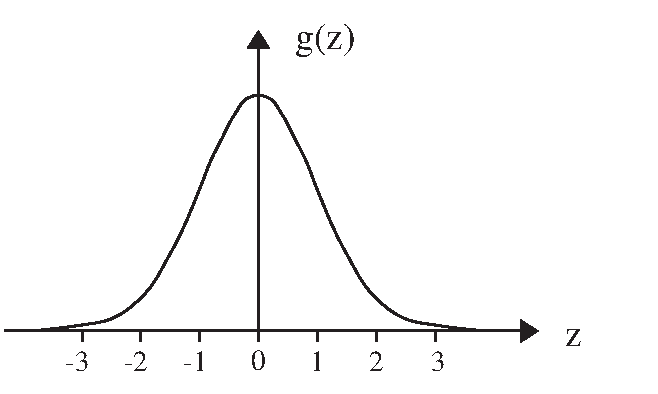
\includegraphics[scale=1.0]{figurer/fig6_1.pdf} 
\caption{Normalkurven}
	\label{fig:Normalkurven}
\end{figure}

\noindent Vi ser at normalkurven har klokkefasong, og er symmetrisk
om null. Det kan også vises at det totale areal som avgrenses av
kurven og $z$-aksen er 1. I statistiske tabellverker finner vi
tabulert (se Tabell~\ref{tab:Normal_Kurvenareal} og ~\ref{tab:Normal_Kurvefraktiler} i Appendiks~\ref{app:fordelngstabeller})

\[ G(z) =  \mbox{\ Arealet under normalkurven til venstre for $z$.} \]

Dette er illustrert i Figur~\ref{fig:arealet_under}.

\begin{figure}[ht]
\centering
	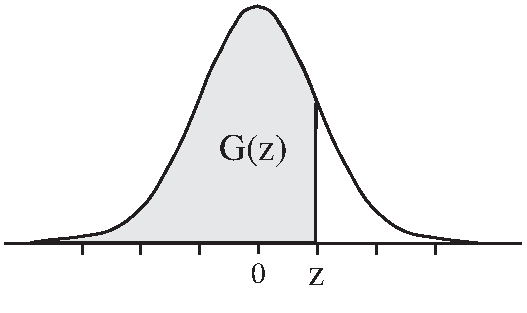
\includegraphics[scale=1.0]{figurer/fig6_2.pdf} 
\caption{Arealer under Normalkurven}
	\label{fig:arealet_under}
\end{figure}

\noindent Vi ser at arealet under normalkurven til høyre for $z$ blir $1 -
G(z)$, mens arealet under normalkurven mellom $u$ og $v$ blir
$G(v) - G(u)$ når $u\leq v$. Siden normalkurven er symmetrisk om
null må vi ha 
\begin{center} \framebox[10cm]{\begin{minipage}{9cm}
\[ \mbox{\ \ \ G1. \ \ \ \ } G(-z)=1-G(z) \]
\mbox{}\vspace{-0.5\belowdisplayskip}
  \end{minipage}} \end{center}
Den siste formelen innebærer at det er nok å tabellere $G(z)$ for
positive argumenter. La oss presentere et utsnitt av Tabell~\ref{tab:Normal_Kurvenareal}:

\begin{center}
\begin{tabular}{c|cccccccc}
  $z$ &  0  & 0.5 & 1.0 & 1.5 & 2.0 & 3.0 &$\cdots$& $\infty$ \\ \hline
$G(z)$&0.500&0.692&0.841&0.933&0.977&0.999&$\cdots$&1.000
\end{tabular}
\end{center}

\noindent Vi skal nå se at normalkurven kan brukes som et hjelpemiddel ved
tilnærmet beregning av sannsynligheter:
La $X$ være en stokastisk variabel med forventning $\mu$ og
varians ${\sigma}^2$. Betrakt den standardiserte variable

\[ Z=\frac{X-\mu}{\sigma} \]

\noindent Anta at histogrammet til $Z$ kan tilnærmes med normalkurven,
som illustrert i Figur~\ref{fig:normal_approx}. Dette vil bl. a. bety at $P(Z\leq z)\approx G(z)$.

\begin{figure}[ht]
\centering
	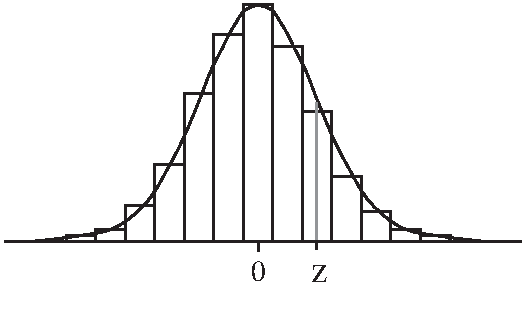
\includegraphics[scale=1.0]{figurer/fig6_3.pdf} 
\caption{Normaltilnærming}
	\label{fig:normal_approx}
\end{figure}

\noindent Siden $P(X \leq x)=P(\frac{X-\mu}{\sigma} \leq \frac{x-\mu}{\sigma})
    =P(Z \leq  \frac{x-\mu}{\sigma})$, får vi formelen

\begin{center} \framebox[10cm]{\begin{minipage}{9cm}
\[ \mbox{\ \ \ G2. \ \ \ \ } P(X \leq x) \approx G(\frac{x-\mu}{\sigma}) \]
\mbox{}  \end{minipage}} \end{center}

\noindent Med en fordeling som kan tilnærmes med normalkurven er det,
for tilnærmet beregning av sannsynligheter, nok å kjenne
forventning og standardavvik. Andre typer sannsynligheter kan
henføres til denne grunnleggende formlen. Ved å bruke
 $P(X > x)=1-P(X \leq x)$ og $P(a < X \leq b)=P(X \leq b)-P(X \leq a)$,
 får vi f.eks.


\begin{center} \framebox[10cm]{\begin{minipage}{9cm}
\[    \mbox{\ \ G3.\ \ \ } P(X > x) \approx 
           1-G(\frac{x-\mu}{\sigma}) \mbox{\ \ \ \ \ \ \ \ \ \ \ \ \ \ \ \ } \]
\[\mbox{\ \ G4. \ \ \ } P(a < X \leq b) \approx  
           G(\frac{b-\mu}{\sigma})-G(\frac{a-\mu}{\sigma}) \]
\mbox{}  \end{minipage}} \end{center}

\noindent I hvilke situasjoner kan vi rettferdiggjøre bruk av
normaltilnærming? \\Følgende situasjon er spesielt viktig:
\begin{center} \framebox[10cm]{\begin{minipage}{9cm}\rule{0cm}{0.5cm}
     Dersom $X$ kan skrives som en sum av et tilstrekkelig stort
     antall uavhengige stokastiske variable med samme
     sannsynlighetsfordeling, så vil histogrammet til 
     $Z=\frac{X-\mu}{\sigma}$ kunne tilnærmes med normalkurven. \\
 \end{minipage}} \end{center} 
\noindent Begrunnelsen for dette ligger delvis i følgende setning:
\begin{center} \framebox[10cm]{\begin{minipage}{9cm}\rule{0cm}{0.5cm}
     {\bf Sentralgrensesetningen :}\\
      Anta at $X_1, X_2, \ldots , X_n$
     er uavhengige stokastiske variable med samme
     sannsynlighetsfordeling, og la 
    \[S_n=X_1+X_2+\cdots +X_n .\]
    Når $n$ vokser mot uendelig vil \footnote{Forutsett at
     forventning og varians eksisterer (jfr. Kapittel 5.8).}
   \[ P(\frac{S_n-ES_n}{\sigma (S_n)} \leq z) \rightarrow G(z) \]
  \end{minipage}} \end{center}
\noindent Under forutsetningene i setningen vil en derfor kunne vente at

   \[ P(\frac{S_n-ES_n}{\sigma (S_n)} \leq z) \approx G(z)  
            \mbox{\ \ for tilstrekkelig stor $n$.}        \]

\noindent Sentralgrensesetningen har hatt en fundamental betydning i
 utviklingen av moderne sannsynlighetsteori, og den har også vidtrekkende
konsekvenser for statistisk praksis. Setningen tilskrives gjerne
Laplace, men et spesialtilfelle av setningen var kjent av De
Moivre \footnote{De Moivre fransk matematiker (1667 - 1754).
Laplace fransk matematiker (1759 - 1827).}). Senere er det
utviklet  mer generelle versjoner av setningen, bl. a. behøver de
stokastiske variable som inngår ikke nødvendigvis ha samme
sannsynlighetsfordeling, visse typer avhengighet tillates også,
men det vil føre for langt å komme inn på disse forhold her. Et
bevis for setningen vil også falle utenfor rammen av denne
framstilling. Vi vil isteden forsøke å gi leseren en viss
forståelse av hvordan et slikt resultat kan oppstå, ved å se på
et eksempel: 

Anta at den felles sannsynlighetsfordeling til $X_i$'ene er gitt
ved $p(x)$ (Se Oppgave~\ref*{kap:stokastiske}.41).

\begin{center}
\begin{tabular}{c|ccc}
 $x$   &  0  &  1  &  2 \\ \hline
 $p(x)$&$\frac{1}{3}$&$\frac{1}{3}$&$\frac{1}{3}$
\end{tabular}
\end{center}
\noindent Sannsynlighetsfordelingen til $S_2=X_1+X_2$ er da
\begin{center}
\begin{tabular}{c|ccccc}
 $s$   &  0  &  1  &  2 &  3  &  4\\ \hline
 $P(S_2=s)$&$\frac{1}{9}$&$\frac{2}{9}$&$\frac{3}{9}$&
                                  $\frac{2}{9}$&$\frac{1}{9}$
\end{tabular}
\end{center}
\noindent mens sannsynlighetsfordelingen til $S_3=X_1+X_2+X_3$ blir
\begin{center}
\begin{tabular}{c|ccccccc}
 $s$   &  0  &  1  &  2 &  3  &  4  &  5  &  6\\ \hline
 $P(S_3=s)$&$\frac{1}{27}$&$\frac{3}{27}$&$\frac{6}{27}$&
                 $\frac{7}{27}$&$\frac{6}{27}$&$\frac{3}{27}$&$\frac{1}{27}$
\end{tabular}
\end{center}
\noindent Histogrammene til $S_1$, $S_2$ og $S_3$ er derfor som vist i
Figur~\ref{fig:hist_k6}.

\begin{figure}[ht]
\centering
	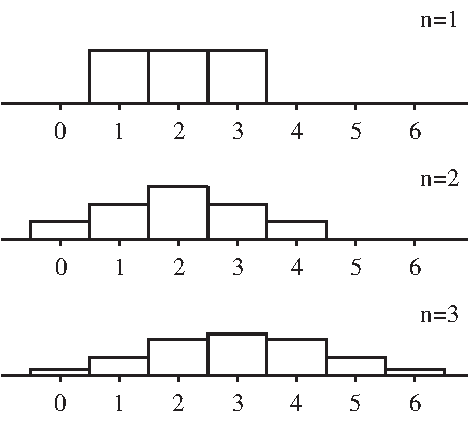
\includegraphics[scale=1.0]{figurer/fig6_4.pdf} 
\caption{Histogrammet til $S_n$}
	\label{fig:hist_k6}
\end{figure}

\noindent Vi har her startet med uavhengige variable med histogram som
slett ikke er klokkeformet, men allerede for $n=3$ viser
histogrammet til $S_n$ trekk av klokkefasong. Vi ser imidlertid
at ettersom $n$ vokser vil histogrammene bli utflytende og det
vanskeliggjør sammenligninger. Dette er en av grunnene til at vi
standardiserer, slik at vi kan sammenligne fordelinger med samme
forventning og varians. Histogrammene til de standardiserte
variable ser ut som i Figur~\ref{fig:hist_standard}.
\clearpage
\begin{figure}[ht]
\centering
   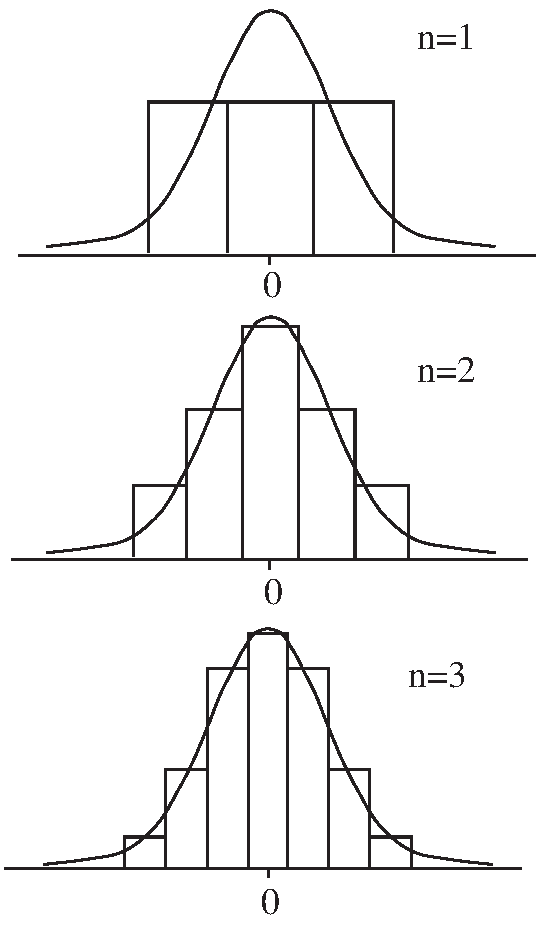
\includegraphics[scale=0.8]{figurer/fig6_5.pdf} 
\caption{Histogrammer til de standardiserte $S_n$}
	\label{fig:hist_standard}
\end{figure}

Vi ser at tendensen mot en klokkeformet kurve er åpenbar, og
dersom vi fortsetter med $n=4, 5, \ldots$, vil vi ytterligere få
bekreftet dette. For stor $n$ vil søylene i histogrammet bli
smale, men til gjengjeld blir det mange av dem, og omrisset av
histogrammet kan etter hvert ikke skjeldnes fra en kontinuerlig
kurve, som altså viser seg å være normalkurven. Det
oppsiktsvekkende er at det er den samme kurven som framkommer
uansett hvilken sannsynlighetsfordeling vi starter med. Selv
dersom vi starter med en fordeling av en helt annen karakter enn
i eksemplet ovenfor vil histogrammene til en sum av uavhengige
variable med denne fordeling nærme seg normalkurven, i den
forstand som er gjort presist i sentralgrensesetningen.
Imidlertid kan en vente at tilnærmingen skjer noe langsommere
dersom vi starter med en U-formet fordeling (Se Oppgave~\ref*{kap:stokastiske}.41
(ii)) eller med en skjev fordeling (Se Oppgave~\ref*{kap:stokastiske}.41 (iii)).
                                    
Før vi ser på anvendelser av normaltilnærming vil vi gjøre noen
merknader: \\

La $X$ være en stokastisk variabel med forventning $\mu$ og
varians ${\sigma}^2$ som er slik at den standardiserte variable
$Z=(X-\mu )/\sigma$ har histogram som kan tilnærmes med
normalkurven. I en rekke anvendelser vil $X$ være en
heltallsvariabel, dvs. $X$ kan bare anta verdier blant de hele
tall. I slike tilfeller vil vi kunne gi en enda bedre tilnærming
enn den vi har i formelen $P(X\leq x)\approx G((x-\mu)/\sigma)$.
La oss studere et utsnitt av histogrammet til $Z$ sammen med et
utsnitt av normalkurven.

\begin{figure}[ht]
\centering
   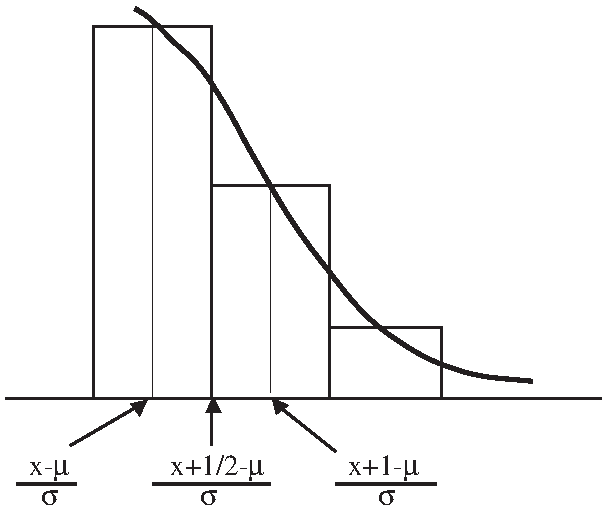
\includegraphics[scale=0.8]{figurer/fig6_6.pdf} 
\caption{Normaltilnærming for heltallsvariable}
	\label{fig:heltalss_koreks}
\end{figure}


I Figur~\ref{fig:heltalss_koreks} er tegnet to søyler sentrert i
to mulige verdier av $Z$, nemlig $(x-\mu)/\sigma$ og $(x+1-\mu)
/\sigma$ der $x$ er heltall. Siden $P(X\leq x)=P(Z\leq (x-\mu)
/\sigma)$ er lik summen av arealene av søylen over $(x-\mu)
/\sigma$ og søylene til venstre for $(x-\mu)/\sigma$, ser vi av
figuren at vi får en bedre tilnærming dersom vi, istedenfor å
beregne arealet under normalkurven til venstre for $(x-\mu)
/\sigma$, beregner arealet til venstre for midtpunktet mellom de
to mulige verdiene, nemlig $(x+\frac{1}{2}-\mu)/\sigma$. Disse
betraktningene har gitt oss følgende tilnærmingsformel

\begin{center} \framebox[10cm]{\begin{minipage}{9cm}
\[ \mbox{\ \ \ G5. \ \ \ \ }   P(X \leq  x) \approx
              G(\frac{x+\frac{1}{2}-\mu}{\sigma})    \]
\mbox{}  \end{minipage}} \end{center}

\noindent Dette kalles {\em normaltilnærming med heltallskorreksjon} og
formelen brukes bare i situasjoner der $X$ er en
heltallsvariabel. Formlene G3 og G4 ovenfor kan i denne situasjon
modifiseres tilsvarende.\\

\begin{eksempel}{Terningkast}
Vi utfører $n$ uavhengige kast med en vanlig terning og lar 

\begin{center}
     $X_i =$ antall øyne i $i$'te kast $i=1,2,\ldots ,n$
\end{center}
\noindent Her blir $X_1, X_2, \ldots , X_n$ uavhengige stokastiske variable med
samme sannsynlighetsfordeling. Vi vet fra før at $EX_i =7/2$, mens
$varX_i =35/12$. Sum øyne i $n$ kast blir

\[ S_n =X_1+X_2+\cdots +X_n \]

\noindent Her blir $ES_n=n\cdot \frac{7}{2}$,
 mens $varS_n=n\cdot \frac{35}{12}$,
slik at når $n$ går mot uendelig vil

\[  P(\frac{S_n-n \cdot \frac{7}{2}}{\sqrt{n \cdot \frac{35}{12}}} \leq z)
                      \rightarrow G(z) \]

\noindent Vi har tidligere tegnet histogrammet til $S_n$ i tilfellet $n=2$.
Dette hadde form av en trekant. Det samme vil være tilfelle for
den standardiserte variable. Allerede for $n=3$ vil histogrammet
få den karakteristiske klokkefasongen (Oppgave~23).
La antall kast $n=4$. Da blir $ES_4=14$ og $varS_4=35/3={(3.4)}^2$.
La oss beregne sannsynligheten for at sum øyne blir høyst 10.
Eksakt beregning gir (tidkrevende opptelling)

\[ P(S_4 \leq 10)=\frac{203}{6^4}=\frac{203}{1296}=0.137 \]

\noindent Tilnærmet beregning (med heltallskorreksjon) gir
\begin{eqnarray*}
P(S_4 \leq 10) \approx G(\frac{10+0.5-14}{\sqrt{35/3}})&=&G(-1.02)=1-G(1.02) \\
                   &=&1-0.846=0.154
\end{eqnarray*}
\noindent dvs. slett ikke verst. Spørsmålet om hva som kan betraktes
 som en brukbar tilnærmelse må vi imidlertid avgjøre i hver konkret
anvendelse, og avhenger selvsagt av formålet med beregningen. \\
\end{eksempel}

\begin{eksempel}{Binomiske sannsynligheter}
Anta at $X$ er binomisk fordelt $(n,p)$. Vi vet da at vi kan
skrive 

\[ X=I_1+I_2+\cdots +I_n \]
\noindent hvor $I_1, I_2, \ldots , I_n$ er indikatorer som oppfyller kravene
til uavhengighet og samme fordeling i sentralgrensesetningen.
Siden $EX=np$ og $varX=np(1-p)$, kan vi slutte at når $n$ går mot
uendelig vil

\[  P(\frac{X-n \cdot p}{\sqrt{np(1-p)}}\leq z) \rightarrow G(z) \]

\noindent La $X=$ antall kron i løpet av 10 myntkast. Da er $X$ binomisk
fordelt $(n=10, p=\frac{1}{2})$. Vi ønsker å beregne
sannsynligheten for høyst 4 kron. Eksakt regning gir

\[ P(X \leq 4)=\frac{386}{1024}=0.377 \]

\noindent Tilnærmet regning gir

\begin{eqnarray*}
P(X \leq 4) \approx G(\frac{4+\frac{1}{2}-10 \cdot \frac{1}{2}}
     {\sqrt{10 \cdot \frac{1}{2} \cdot \frac{1}{2}}})&=&G(-0.317)=1-G(0.317)\\
                   &=&1-0.624=0.376
\end{eqnarray*}

\noindent Anta at det isteden er tale om $n=100$ myntkast, og vi ønsker
 å beregne sannsynligheten for høyst 40 kron. Siden de fleste
tabeller over den binomiske fordeling ikke går så langt som til
$n=100$, er vi nødt å ty til normaltilnærmelse. Vi får

\begin{eqnarray*}
P(X \leq 40) \approx G(\frac{40+0.5-50}
     {\sqrt{100 \cdot \frac{1}{2} \cdot \frac{1}{2}}})&=&G(-1.9)=1-G(1.9)\\
                   &=&1-0.971=0.029
\end{eqnarray*}

\noindent For beregning av binomiske sannsynligheter ved hjelp av
normaltilnærming vil vi gi en {\em tommelfingerregel:}
Normaltilnærming gir som regel godt resultat når $np(1-p) \geq 10$,
 brukbart for $np(1-p) \geq 5$. \\
\end{eksempel}

\begin{eksempel}{Hypergeometriske sannsynligheter}
Anta at $Y$ er hypergeometrisk fordelt $(N,M,n)$. Vi har sett at
vi kan skrive

\[   Y=I_1+I_2+\cdots +I_n \]

\noindent der $I_1, I_2, \ldots , I_n$ er indikatorer med samme
sannsynlighetsfordeling, men som er avhengige, slik at kravet i
sentralgrensesetningen ikke er oppfylt. Dersom $n$ er liten i
forhold til $N$, vet vi at $I_1, I_2, \ldots , I_n$ er tilnærmet
uavhengige. I en slik situasjon kan vi, dersom vi ikke kommer
fram på annen måte, likevel bruke normaltilnærming med brukbart
resultat. La oss ta et konkret eksempel: \\
I en forening på $N=1000$ medlemmer er det $M=500$ kvinner og $N-
M=500$ menn. Det trekkes et tilfeldig utvalg på $n=100$ medlemmer
som inviteres til jubileumsmiddag. La $Y$ være antall kvinner i
utvalget. Vi ønsker å beregne sannsynligheten for at det
inviteres færre kvinner enn menn, dvs. høyst 49 kvinner, samt
sannsynligheten for at det inviteres høyst 45 kvinner. Vi ser at
$Y$ er hypergeometrisk fordelt $(N=1000, M=500, n=100)$. Her blir
 $EY=n \cdot \frac{M}{N}=50$ og $varY=\frac{N-n}{N-1} \cdot n \cdot
    \frac{M}{N} \cdot (1-\frac{M}{N})=22.5$
Vanlige tabeller strekker ikke til. Siden $n$ er stor, men
likevel relativt liten i forhold til $N$, forsøker vi
normaltilnærming:

\begin{eqnarray*}
P(Y \leq 49) \approx G(\frac{49+0.5-50}{\sqrt{22.5}})&=&G(-0.105)=1-G(0.105)\\
                 &=&1-0.542=0.458 \\
P(X \leq 45) \approx G(\frac{45+0.5-50}{\sqrt{22.5}})&=&G(-0.949)=1-G(0.949)\\
                   &=&1-0.829=0.171
\end{eqnarray*}

\noindent Av et større tabellverk finner vi de eksakte sannsynligheter, men
de er ikke nevneverdig forskjellig fra de tilnærmede.
\end{eksempel}

\begin{eksempel}{Poissonsannsynligheter}
Anta at $X$ er Poissonfordelt med forventning $\lambda$. Dersom
$\lambda$ er stor kan vi benytte normaltilnærming. Dette er ikke
like lett å begrunne som i de to foregående eksemplene. Det
faktum at Poissonsannsynligheter kan oppnås som grense for
binomiske sannsynligheter for voksende $n$, og at binomiske
sannsynligheter kan tilnærmet beregnes ved bruk av normalkurven
for stor $n$, antyder at normaltilnærming kan være aktuelt også
her. Et annet argument: I situasjoner der $\lambda$ er heltall
kan vi skrive (se Oppgave~37)

\[  X=X_1+X_2+\cdots +X_{\lambda} \]

\noindent der $X_i$'ene er uavhengige og $X_i$ Poissonfordelt med
forventning $1$. Vi kan med referanse til
sentralgrensesetningen slutte at når $\lambda$ går mot uendelig vil

\[  P(\frac{X- \lambda}{\sqrt{\lambda}}\leq z) \rightarrow G(z) \]

\noindent Vi ser at Tabell~\ref{tab:Poisson_fordeling} ikke går lenger enn til $\lambda =10.0$. For
$\lambda \geq 10.0$ vil normaltilnærming gi brukbart resultat for
de fleste praktiske formål. La oss ta et eksempel: Anta at antall
ordrer på en bestemt vare pr. dag er Poissonfordelt med
forventning $\lambda =10.0$. Da blir eksempelvis

\[P(X \leq 8) \approx G(\frac{8+0.5-10}{\sqrt{10}})=G(-0.4743)=0.318 \]

\noindent mens det korrekte resultat er 0.333. \\
\end{eksempel}
Noen sluttkommentarer om normaltilnærming: \\
Anta fortsatt at histogrammet til $Z=(X-\mu )/\sigma$ kan tilnærmes
med normalkurven, og la $A(k)$ være arealet under normalkurven
mellom $-k$ og $k$. Dette kan beregnes ved
\[ A(k)=G(k)-G(-k)=G(k)-(1-G(k))=2G(k)-1. \]
\noindent Vi får

\begin{center} \framebox[10cm]{\begin{minipage}{9cm}
\[ \mbox{\ \ \ G6. \ \ \ \ } P(\mid X-\mu \mid < k\cdot \sigma)\approx A(k)  \]
\mbox{}  \vspace{-0.5\belowdisplayskip}
  \end{minipage}} \end{center}

\noindent dvs. at sannsynligheten for at $X$ faller innenfor $k$ ganger
standardavviket fra sin forventning er entydig (tilnærmet) gitt ved $k$. La
oss gi noen verdier
\begin{center}
\begin{tabular}{c|cccc}
 $k$&  0.5  &  1.0  &  2.0  &  3.0 \\ \hline
 $A(k)$&0.38&0.68&0.95&0.99  
\end{tabular}
\end{center}
\noindent Ved å sette $k=d/\sigma$ i formelen ovenfor får vi en
 alternativ formel

\begin{center} \framebox[10cm]{\begin{minipage}{9cm}
\[ \mbox{\ \ \ G7. \ \ \ \ } P(\mid X-\mu \mid < d)\approx
                                             A(\frac{d}{\sigma}) \]
\mbox{}   \end{minipage}} \end{center}

\noindent Vi ser at når standardavviket $\sigma$ er kjent, vil vi kunne
beregne tilnærmet sannsynligheten for at $X$ faller innenfor et
bestemt antall enheter $d$ fra sin forventning, dvs. $\sigma$ kan
direkte relateres til risiko. \\


\begin{eksempel}{Tegnestiften}
La sannsynligheten være $p$ for at en tegnestift faller med
spissen opp ved et kast, og la $X$ være antall ganger den peker
opp i $n$ uavhengige kast, slik at $X$ er binomisk fordelt
$(n,p)$. Betrakt sannsynligheten

\[ P(\mid \frac{X}{n}-p \mid < k \cdot \sigma (\frac{X}{n})) \mbox{\ \ der \ }
                        \sigma (\frac{X}{n})=\sqrt{\frac{p(1-p)}{n}} .\]

\noindent Ifølge teorien ovenfor blir denne sannsynligheten tilnærmet
 lik $A(k)$. Det vil være instruktivt å beregne $\sigma$ for noen
verdier av $n$ og $p$. Siden $p$ trolig ligger i området omkring
$0.5$, nøyer vi oss med noen få $p$-verdier \footnote{Merk at
$\sigma $ varierer lite i området omkring $p=0.5$, for øvrig vil
$p$ alltid gi samme $\sigma$ som $p'=1-p$.}

\begin{center}
\begin{tabular}{c|ccccc}
 $p$   & $n=$& 100 & 500 &1 000&10 000 \\ \hline
 0.4   &     &0.049&0.021&0.015&0.0049 \\
 0.5   &     &0.050&0.022&0.016&0.0050 \\
 0.6   &     &0.049&0.021&0.015&0.0049 \\ \hline
\end{tabular}
\end{center}
\noindent Av denne tabellen (og tabellen ovenfor) kan vi f.eks. slutte at
når $n=1000$ er sannsynligheten for at hyppigheten avviker fra
sannsynligheten $p$ med mindre enn $0.016$ tilnærmet lik $0.68$,
mens sannsynligheten for at hyppigheten avviker mindre enn
$2\cdot 0.016=0.032$ er tilnærmet lik $0.95$. Dette eksemplet
belyser fra en teoretisk synsvinkel de forhold som ble diskutert
i Eksempel 2 i Kapittel 1, hvor vi søkte å motivere
sannsynlighetsbegrepet.
\end{eksempel}


\section{Tsjebysjeffs ulikhet. Store talls lov.}

I slutten  av forrige avsnitt så vi at standardavviket er svært
informativt i situasjoner hvor normaltilnærming er brukbar.
Følgende setning viser imidlertid at standardavviket til en viss
grad også er informativt i mer generelle situasjoner.

\begin{center} \framebox[10cm]{\begin{minipage}{9cm}\rule{0cm}{0.5cm}
     {\bf Tsjebysjeffs ulikhet :} 
\footnote{Oppkalt etter den russiske matematiker Tsjebysjeff (1821 - 1894).} \\
     La $X$ være en stokastisk
     variabel med forventning $\mu$ og standardavvik $\sigma$. Da er
\[ P(\mid X-\mu \mid < k \cdot \sigma) \geq 1- \frac{1}{k^2} 
                      \mbox{\ \ (for $k \cdot \sigma > 0)$.} \] 
  \end{minipage}} \end{center}

\noindent Dette viser at uansett sannsynlighetsfordelingen til $X$ så gir
ulikheten  en nedre skranke $1-1/k^2$
 for sannsynligheten for avvik i tallverdi mindre enn $k$
ganger standardavviket fra forventningen. Denne skranken er for
noen verdier av $k$

\begin{center}
\begin{tabular}{c|cccccc}
     $k$   &  1  &  2   &  3  &  4  &  5  &  $\cdots$ \\ \hline
 $1-1/k^2$ & 0.00& 0.75 & 0.88& 0.94& 0.96 & $\cdots$
\end{tabular}
\end{center}
\noindent For en gitt sannsynlighetsfordeling vil vanligvis de eksakte
sannsynlighetene være betydelig høyere, men tabellen gir altså
garanterte verdier som kan nyttes også i situasjoner hvor vi ikke
kjenner sannsynlighetsfordelingen i detalj.

\small
\noindent Begrunnelse for Tsjebysjeffs ulikhet: Vi ser at det er nok å
 vise at 

\[   P(\mid Z\mid < k) \geq 1-1/k^2 \]

\noindent der $Z=(X-\mu)/\sigma$ er den standardiserte variable til $X$.
Definer en ny stokastisk variabel $Y$ ved at
\begin{eqnarray*}
     Y&=&0  \mbox{\ \ \ \ dersom \ } \mid Z\mid < k \\
      &=&k^2 \mbox{\ \ \ dersom \ } \mid Z\mid \geq k
\end{eqnarray*}
\noindent Da er $Y\leq Z^2$ og følgelig også $EY\leq EZ^2=varZ=1$.
 Men nå er 

\[ EY=0 \cdot P(\mid Z \mid < k)+k^2 P( \mid Z \mid \geq k). \]

\noindent Følgelig blir $k^2 P( \mid Z \mid \geq k) \leq 1$,
 eller med andre ord

\[     P(\mid Z \mid \geq k) \leq 1/k^2 \]

\noindent som er ekvivalent med det søkte resultat.\\
\normalsize

\begin{eksempel}{Tennsatsen}
En produsent lager tennsatser og har erfart at brenntiden til en
tennsats kan oppfattes som en stokastisk variabel $X$ med
forventning $5.0$ og standardavvik $0.2$. Da er eksempelvis

\[ P( \mid X-5.0 \mid < 1.0) \geq 0.96, \]

\noindent uansett hvilken sannsynlighetsfordeling $X$ har.
\end{eksempel}

En variant av Tsjebysjeffs ulikhet får vi ved å
sette $d=k \cdot \sigma$, dvs.

\[P( \mid X-\mu \mid < d)\geq 1-\frac{{\sigma}^2}{d^2}\mbox{\ \ (for $d>0$).}\]

\noindent En interessant anvendelse av denne har vi i den binomiske situasjon:\\

Anta at $X$ er binomisk fordelt $(n,p)$, og la oss anvende den
siste ulikheten på den relative hyppighet av suksesser i de $n$
forsøk. Siden $E(X/n)=p$ og $var(X/n)=p(1-p)/n$, får vi

\[ P(\mid \frac{X}{n}-p \mid < d) \geq 1- \frac{p(1-p)}{nd^2} . \]

\noindent Vi ser at den garanterte nedre skranke for sannsynligheten for at
den relative hyppighet av suksesser avviker fra sannsynligheten
$p$ med mindre enn $d$, vokser med $n$ for gitt $d>0$. Vi ser at
vi faktisk kan konkludere at 

\[ P(\mid \frac{X}{n}-p \mid < d) \rightarrow 1 \mbox{\ \ når \ }
                 n \rightarrow \infty \]

\noindent uansett $d>0$. I denne forbindelse sies ofte at den relative
hyppighet {\em konvergerer} mot $p$ i {\em sannsynlighet}. Dette
resultat omtales ofte som {\em Bernoullis lov om de store tall}
\footnote{Oppkalt etter Jakob Bernoulli (1654 - 1705).}, og er
en slags teoretisk bekreftelse på at sannsynligheter kan framkomme som
idealiserte relative hyppigheter i det lange løp (Se Kapittel 1).


\section{$\star$Den geometriske fordeling}
\small
Anta at vi har en binomisk forsøksrekke med suksess-sannsynlighet
$p$, og la

\[N= \mbox{\ \ ventetiden til første suksess.} \]

\noindent I Kapittel 4.6 fant vi at 

\[ p(n)=P(N=n)={(1-p)}^{n-1} \cdot p \; \; ; \; n=1,2,3,\ldots \]

\noindent Denne sannsynlighetsfordelingen kalles {\em den geometriske
fordeling}. Ifølge summeformelen for en geometrisk rekke får vi

\[ \sum_np(n)=p\sum_{n=1}^{\infty}{(1-p)}^{n-1}=p({(1-(1-p))}^{-1}=1 \]

\noindent som viser at vi virkelig har en sannsynlighetsfordeling. Vi
ønsker å beregne forventningen til $N$. Vi får

\[ EN=\sum_nnp(n)=p\sum_{n=1}^{\infty}n{(1-p)}^{n-1}=\frac{1}{p} \]

\noindent Begrunnelse: La for enkelhets skyld $q=1-p$ og betrakt

\begin{eqnarray*}
 (1-q)\sum_{n=1}^{\infty}nq^{n-1}&=&
                 \sum_{n=1}^{\infty}nq^{n-1} - \sum_{n=1}^{\infty}nq^n \\
 &=&\sum_{n=1}^{\infty}nq^{n-1}-\sum_{n=2}^{\infty}(n-1)q^{n-1}\\
 &=&1+\sum_{n=2}^{\infty}q^{n-1}=1+q{(1-q)}^{-1}=p^{-1}
\end{eqnarray*}
\noindent Eksempler på anvendelser av dette resultat er: Forventet ventetid
til første kron i myntkast ($p$=1/2) blir 2. Forventet
ventetid til første sekser i terningkast ($p$=1/6) blir 6.
Forventet ventetid til første defekt når defektsannsynligheten er
$p=0.05$ blir $20$.

Variansen til en geometrisk fordelt stokastisk variabel $N$ viser
seg å bli $varN=q/p^2$. Denne utledning er noe mer komplisert, og
siden resultatet ikke har så stor praktisk interesse, utelater vi
begrunnelsen her. Vi vil isteden rette oppmerksomheten mot en
interessant egenskap ved den geometriske fordeling.
La oss først finne sannsynligheten for at ventetiden til første
suksess er mer enn $k$

\[ P(N > k)=\sum_{n=k+1}^{\infty}p(n)
            =p\sum_{n=k+1}^{\infty}{(1-p)}^{n-1}={(1-p)}^k \]

\noindent Gitt at ventetiden er minst $k$, da er sannsynligheten for at
vi må vente $n$ tidsenheter til før første suksess:
\begin{eqnarray*}
P(N=k+n \mid N>k)&=&\frac{P(N=k+n)}{P(N>k)} \\
                 &=&\frac{{p(1-p)}^{k+n-1}}{{(1-p)}^k}=p{(1-p)}^{n-1}
\end{eqnarray*}
\noindent som jo er det samme som $P(N=n)$. dette betyr at gjenstående
ventetid er upåvirket av hvor lenge vi allerede har ventet, vi
sier at den geometriske fordeling er uten minne. Dette er kanskje
ikke så overaskende når vi tenker på at vi har utledet den
geometriske fordeling fra en serie med uavhengige binomiske
forsøk. Det kan vises at den geometriske fordeling er den eneste
diskrete fordeling som er uten minne.
\normalsize


\section{$\star$Den multinomiske fordeling}
\small

Vi husker at en binomisk forsøksrekke var en rekke uavhengige
forsøk der hvert forsøk hadde to mulige utfall og der
sannsynlighetene for disse utfallene var den samme i alle
forsøkene. I dette avsnittet vil vi se på en tilsvarende
situasjon, men hvor det kan foreligge mer enn to mulige utfall i
hvert forsøk. \footnote{I det følgende forutsettes det at leseren
er kjent med stoffet i Kapittel 3.7 om gruppering.})
Det utføres en rekke eksperimenter (forsøk) hvor:
\begin{enumerate}
\item Hvert forsøk gir et av $m$ mulige utfall $u_1, u_2, \ldots , u_m$.
\item Sannsynlighetene for hvert av de mulige utfallene er de
     samme i alle forsøk.
\item Forsøkene er uavhengige.
\end{enumerate}
Denne situasjon kaller vi en {\em multinomisk forsøksrekke.}

Vi ser at tilfellet $m=2$ svarer til binomisk forsøksrekke.
Tilfellet $m=3$ kalles ofte en trinomisk forsøksrekke.
Eksempelvis har vi tidligere sett at i en løpende produksjon hvor
hver produsert artikkel blir klassifisert som intakt $(i)$ eller
defekt $(d)$ kan betraktes som en binomisk forsøksrekke. Dersom
intakte artikler klassifiseres i tre kvaliteter (a, b og c) kan
produksjonen betraktes som en multinomisk forsøksrekke med $m=4$
mulige resultater i hvert forsøk. Vi må da være villige til å
anta uavhengighet og samme sannsynlighet for de ulike
kvalitetskategorier for alle forsøk.

Anta at vi utfører $n$ multinomiske forsøk og anta at
sannsynligheten for at utfallene $u_1, u_2, \ldots , u_m$ observeres
i et enkelt forsøk er henholdsvis $p_1, p_2, \ldots , p_m$ hvor
$p_1+p_2+\cdots +p_m =1$. Vi ønsker å beregne sannsynligheten for
at
\begin{center}
\begin{tabular}{l}
     $u_1$ observeres $x_1$ ganger\\
     $u_2$ observeres $x_2$ ganger\\
     $\vdots $                     \\
     $u_m$ observeres $x_m$ ganger, der $x_1+x_2+\cdots +x_m=n$.
\end{tabular}
\end{center}
\noindent La derfor for $i=1, 2, \ldots , m$

\[ X_i= \mbox{\ \ antall ganger resultatet $u_i$ observeres.} \]

\noindent Det viser seg at den simultane sannsynlighetsfordelingen til
$X_1, X_2, \ldots , X_m$ er gitt ved sannsynlighetsfunksjonen:

\begin{eqnarray*}
 p(x_1,x_2,\ldots ,x_m)&=&P((X_1=x_1)\cap (X_2=x_2)\cap \cdots (X_m=x_m)) \\
&=&\frac{n!}{x_1!x_2!\cdots x_m!}p_1^{x_1}p_2^{x_2}\cdots p_m^{x_m}
\end{eqnarray*}

\noindent for alle heltall $x_1, x_2, \ldots, x_m$ slik at $x_1+x_2+\cdots
+x_m=n$, mens $p(x_1, x_2, \ldots, x_m)=0$ for alle andre $x_1, x_2,
\ldots, x_m$. Dette kalles {\em den multinomiske
sannsynlighetsfordeling}, og vi sier at $(X_1, X_2, \ldots, X_m)$ er
multinomisk fordelt med parametre $(n, p_1, p_2, \ldots, p_m)$.

En begrunnelse for dette resultatet kan gis i analogi med den vi ga
i den binomiske situasjon: Vi vil først finne ut hvor mange
utfallssekvenser som er slik at $u_1$ forekommer $x_1$ ganger,
$u_2$ forekommer $x_2$ ganger, $\ldots, u_m$ forekommer $x_m$
ganger. Vi tenker oss de $n$ forsøkene nummerert fra $1$ til $n$
og det søkte antall kan finnes ved å telle opp antall måter å
velge ut $x_1$ plasser (numre) som skal gis symbolet $u_1, x_2$
plasser som skal gis symbolet $u_2, \ldots, x_{m-1}$ plasser som
skal gis symbolet $u_{m-1}$, mens de resterende $x_m=n-(x_1+x_2+
\cdots +x_{m-1})$ plassene gis symbolet $u_m$. Dette er
likeverdig med å spørre om antall måter å dele opp populasjonen
bestående av tallene $1, 2, \ldots, n$ i $m$ benevnte grupper med
henholdsvis $x_1$ elementer i gruppe nr.$1$ ($u_1$-gruppen),
$x_2$-elementer i gruppe nr.$2$ ($u_2$-gruppen), $\ldots, x_m$
elementer i gruppe nr.$m$ ($u_m$-gruppen). I Kapittel 3.7 viste
vi at dette antall var lik

\[ \bino{n}{x_1,x_2,\ldots ,x_{m-1}}=\frac{n!}{x_1!x_2!\cdots x_m!}.\] 

\noindent På grunn av uavhengigheten og forutsetningen om samme
sannsynlighet i alle $n$ forsøk, følger at hver av disse
utfallssekvensene har sannsynlighet som er et produkt av $n$
faktorer, hvor $x_1$ faktorer er lik $p_1, x_2$ faktorer lik
$p_2, \ldots, x_m$ faktorer lik $p_m$. Det er bare rekkefølgen av
faktorene som er forskjellig for de ulike utfallssekvensene. Alle
får derfor sannsynlighet

\[   p_1^{x_1}p_2^{x_2}\cdots p_m^{x_m} \]

\noindent som viser at den oppgitte formel er korrekt.\\

\noindent {\bf Merknad.} Den multinomiske fordeling slik den er angitt
ovenfor er en simultan fordeling for $m$ stokastiske variable
$X_1, X_2, \ldots, X_m$. Egentlig er dimensjonen bare $m-1$ fordi
$X_m=n-(X_1+\cdots +X_{m-1})$ og $p_m=1-(p_1+\cdots +p_{m-1})$,
slik at fordelingen er fullstendig beskrevet ved at

\begin{eqnarray*}
 p(x_1,\ldots ,x_{m-1})&=&P((X_1=x_1)\cap \cdots \cap (X_{m-1}=x_{m-1})) \\
&=&\frac{n!}{x_1!\cdots x_{m-1}!(n-(x_1+x_2+\cdots +x_{m-1}))!} \\
& \cdot & p_1^{x_1}\cdots p_{m-1}^{x_{m-1}}{(1-(p_1+\cdots +p_{m-1}))}^{n-(x_1+\cdots +x_{m-1})}
\end{eqnarray*}

\noindent Vi ser at den første skrivemåten gir en mer attraktiv formel,
og som regel brukes den, unntatt er tilfellet $m=2$ hvor den
binomiske fordeling vanligvis skrives som en fordeling i en
dimensjon.\\

\begin{eksempel}{Tolv terningkast}
Vi utfører $n=12$ terningkast. Hvert kast har seks mulige utfall,
et øye $(u_1)$ to øyne $(u_2)$, \ldots, seks øyne $(u_6)$. En
rettferdig terning svarer til at $p_1=p_2=\cdots =p_6=1/6$. Antar
vi at kastene er uavhengige, er vi i en multinomisk situasjon. La
for $i=1, 2, \ldots, 6$

\[ X_i= \mbox{\ \ antall ganger i øyne observeres.} \]

\noindent Da blir sannsynlighetsfordelingen til $X_1, X_2, \ldots, X_6$

\[ p(x_1,x_2,\ldots ,x_6)=\frac{12!}{x_1!x_2!\cdots x_6!}
 {(\frac{1}{6})}^{x_1}\cdot {(\frac{1}{6})}^{x_2}\cdots {(\frac{1}{6})}^{x_6}\]

\noindent for heltall $x_1, x_2, \ldots, x_6$ slik at $x_1+x_2+\cdots+x_6=12$.
Sannsynligheten for at alle øyne forekommer to ganger blir
eksempelvis

\[ p(2,2,\ldots ,2)=\frac{12!}{{(2!)}^6}{(\frac{1}{6})}^{12}=0.0034 \]
\end{eksempel}

\begin{eksempel}{Ti kast med to mynter}
Vi utfører $n=10$ omganger med myntkast med to mynter. I hver
omgang observerer vi resultatet ingen kron $(u_1)$, en kron og en
mynt $(u_2)$ eller to kron $(u_3)$. En rettferdig mynt svarer til
at $p_1=1/4, p_2=1/2$ og $p_3=1/4$. Antar vi at omgangene er
uavhengige er vi i en multinomisk situasjon. La $X_i$ være antall
ganger $u_i$ observeres $(i=1,2,3)$. Da blir
sannsynlighetsfordelingen til $X_1$, $X_2$ og $X_3$

\[ p(x_1,x_2,x_3)=\frac{10!}{x_1!x_2!x_3!}
 {(\frac{1}{4})}^{x_1}\cdot {(\frac{1}{2})}^{x_2}\cdot {(\frac{1}{4})}^{x_3}\]

\noindent for heltall $x_1, x_2, x_3$ slik at $x_1+x_2+x_3=10$.
Sannsynligheten for at vi observerer 3 omganger med begge kron, 4
omganger med en hver og 3 omganger med begge mynt er derfor

\[ p(3,4,3)=\frac{10!}{3!4!3!}
      {(\frac{1}{4})}^3\cdot {(\frac{1}{2})}^4\cdot {(\frac{1}{4})}^3=0.0641\]
\end{eksempel}

\begin{eksempel}{Tipperekke}
En tipperekke i fotball består av $n=12$ kamper, hver kamp har
som mulige utfall hjemmeseier (H), uavgjort (U) eller borteseier
(B). I løpet av en lengre tidsperiode er det observert ca. 45\%
hjemmeseire, 25\% uavgjorte og 30\% borteseire. (Tallene er
konstruerte.) La $X_1$, $X_2$ og $X_3$ betegne henholdsvis antall
hjemmeseire, uavgjorte og borteseire i kommende spilleuke. Er vi
villige til å anta forutsetningene om uavhengighet og samme
sannsynlighet for alle kampene på kupongen (diskuter om dette er
realistisk), er det rimelig å arbeide ut fra at $(X_1, X_2, X_3)$
er multinomisk fordelt $(n=12, p_1=0.45, p_2=0.25, p_3=0.30)$
dvs. 

\[ p(x_1,x_2,x_3)=\frac{12!}{x_1!x_2!x_3!}0.45^{x_1}\cdot 0.25^{x_2}\cdot 
                                                     0.30^{x_3}       \]

\noindent Ut fra dette vil vi kunne finne sannsynlighetene for ulike
tegnfordelinger. Eksempelvis blir

\[ p(6,2,4)=\frac{12!}{6!2!4!}0.45^6\cdot 0.25^2\cdot 0.30^4=0.0582 \]
                            
\noindent Diskuter påstanden: ``Det lønner seg å satse på
 bestemte tegnfordelinger i tipping da noen tegnfordelinger har vist seg å
forekomme oftere enn andre''.
\end{eksempel}

Anta at $(X_1, X_2, \ldots, X_m)$ er multinomisk fordelt med
parametre $(n, p_1, p_2, \ldots, p_m)$. Da vil , for $i=1, 2, \ldots,
m, X_i$ være binomisk fordelt med parametre $(n,p_i)$. Dette
innses direkte ved å notere resultatet $u_i$ som suksess og
ikke-$u_i$ som fiasko. Dette viser at

\[          EX_i=np_i    \]
\[          varX_i=np_i(1-p_i). \]

\noindent Det er imidlertid klart at $X_1, X_2, \ldots, X_m$ ikke kan være
uavhengige. Det viser seg at

\[ cov(X_i, X_j)=-np_ip_j \mbox{\ \ for \ } i\not= j \]

\noindent dvs. som rimelig er negativt korrelerte. Dette innses enklest
slik: La oss notere suksess dersom $u_i$ eller $u_j$ inntreffer,
dette har sannsynlighet $p_i+p_j$. Antall suksesser $X_i+X_j$
blir da binomisk fordelt med parameter $(n,p_i+p_j)$, slik at

\[     var (X_i+X_j)=n(p_i+p_j)(1-(p_i+p_j)). \]

\noindent Men nå er ifølge formel V8

\[     var(X_i+X_j)=varX_i+varX_j+2cov(X_i, X_j), \]

\noindent slik at

\begin{eqnarray*}
cov(X_i, X_j)&=&\frac{1}{2}[n(p_i+p_j)(1-(p_i+p_j))\\
             & &-np_i(1-p_i)-np_j(1-p_j)]=-np_ip_j.
\end{eqnarray*}
\noindent Kunnskaper om den multinomiske fordeling er nyttig i en rekke
forbindelser både i rene sannsynlighetsteoretiske anvendelser og
i statistisk praksis, bl.a. ved test av om en gitt
sannsynlighetsmodell er realistisk, og ved analyse av såkalte
kategoridata.
\normalsize

\section{Oppgaver}
\small
\begin{enumerate}
\item La $X$ være binomisk fordelt $(n,p)$. Bruk tabeller til å
     finne følgende sannsynligheter:
     \begin{itemize}
     \item[(a)]  $P(X=3)$, $P(X\leq 2)$ og $P(X\geq 4)$ når \\
          $n=5$ og $p=0.2, 0.4, 0.5$ og $0.6$,
     \item[(b)]  $P(X=6)$, $P(X\leq 4)$ og $P(X\geq 8)$ når \\
          $n=10$ og $p=0.2, 0.4, 0.5$ og $0.6$,
     \item[(c)]  $P(X=12)$, $P(X\leq 8)$ og $P(X\geq 16)$ når \\
          $n=20$ og $p=0.5$.
     \end{itemize}

\item La $X$ være binomisk fordelt $(n,p)$. Hvilken verdi er mest
     sannsynlig dersom
     \begin{itemize}
     \item[(a)]  $n$=5 og $p$=0.1, 0.2, 0.3, 0.4 og 0.5,
     \item[(b)]  $n$=10 og $p$=0.1, 0.2, 0.3, 0.4 og 0.5.
     \end{itemize}

\item En produksjonsprosess gir 5\% defekte når den er i
     ``kontroll''. De 10 siste artiklene som produseres hver dag
     kontrolleres og antall defekte $X$ noteres. Maskinene
     justeres dersom antall defekte er 3 eller større. Hva er
     sannsynligheten for justering dersom
     \begin{itemize}
     \item[(a)]  prosessen fortsatt er i kontroll,
     \item[(b)]  prosessen er ute av kontroll og gir nå gjennomgående
                 10\%  defekte.
     \end{itemize}

\item En fabrikant av syltetøy vil undersøke om en ny
     konserveringsmetode gir endret smak på produktet. Ti
     personer får smake på 5 smaksprøver hvorav bare en er
     produsert med den nye metode, og de blir bedt om å velge ut
     en prøve som de mener smaker ulikt de andre. Finn
     sannsynligheten for at antall korrekte identifikasjoner av
     det nye produkt er
     \begin{center}
     (a) høyst to  \ \ \ (b) minst tre \ \ \ (c) minst fire
     \end{center}
     under forutsetning av at smaken er uendret og smakerene
     velger tilfeldig. Hva er da forventet antall korrekte
     identifikasjoner?

\item Betrakt et tilfeldig $n$-sifret tall.
     \begin{itemize}
     \item[(a)]  Hva menes med et slikt tall?
     \item[(b)]  Hva blir forventet antall nuller?
     \item[(c)]  Hva blir forventet antall ulike sifre?
     \end{itemize}

\item Et produksjonsparti på $N$ artikler inneholder $M$ defekte.
     Et tilfeldig utvalg på $n$ artikler trekkes ut og antall
     defekte $Y$ noteres. Lag tabeller over
     sannsynlighetsfordelingen til $Y$ i følgende situasjoner:
     \begin{itemize}
     \item[(a)]  $N$=10 $M$=2 $n$=2 \ \ \ (b)  $N$=10 $M$=2 $n$=3
     \item[(c)]  $N$=10 $M$=2 $n$=4 \ \ \ (d)  $N$=10 $M$=3 $n$=2
     \item[(e)]  $N$=10 $M$=3 $n$=3 \ \ \ (f)  $N$=10 $M$=3 $n$=4.
     \end{itemize}
      Hva er forventet antall defekte i utvalget i hver av disse
     situasjonene?
\item  \begin{itemize}
     \item[(a)]  I en pokerhånd på 5 kort finn forventet antall \\
          (i) ess (ii) spar (iii) sorte kort
     \item[(b)]  I en bridgehånd på 13 kort finn forventet antall \\
          (i) ess (ii) spar (iii) sorte kort (iv) honnører
     \end{itemize}

\item Et produksjonsparti består av $N$ artikler hvorav $M$ er
     defekte. Det trekkes ut tilfeldig $n$ artikler for kontroll.
     Bruk tilnærming til binomisk fordeling til å finne tilnærmet
     sannsynligheten for at utvalget inneholder minst to defekte
     i følgende situasjoner:\\
     \begin{tabular}{clllclll}
     (a) &  $N$=100& $M$=5 & $n$=5 & (b) & $N$=100 & $M$=5 & $n$=10 \\
     (c) &  $N$=100& $M$=5 & $n$=15& (d) & $N$=1000& $M$=50& $n$=5 \\
     (e) &  $N$=1000&$M$=50& $n$=10& (f) & $N$=1000& $M$=50& $n$=15.
     \end{tabular} \\
     I et større tabellverk over hypergeometriske sannsynligheter
     finner vi følgende eksakte sannsynligheter
     \begin{itemize}
     \item[(a)]  0.0190 \ \   (b)  0.0769 \ \     (c) 0.1609.
     \end{itemize}
     Kommenter resultatene ovenfor i lys av dette.

\item  La $Y$ være hypergeometrisk fordelt $(N,M,n)$. Vis at vi kan
     la $M$ og $n$ bytte plass og likevel ha samme fordeling.
     Forklar hvordan dette kan utnyttes ved binomisk tilnærming
     for, i visse situasjoner, å oppnå et bedre resultat.


\item  Diskuter om en Poissonmodell kan være realistisk i
     følgende situasjoner:
     \begin{itemize}
     \item[(a)]  oppringninger til et sentralbord,
     \item[(b)]  emisjon av radioaktive partikler,
     \item[(c)]  bakterier i drikkevann,
     \item[(d)]  tidspunkt for ``blow out'' i oljeboring i Nordsjøen,
     \item[(e)]  fotballspillere på en bane,
     \item[(f)]  trykkfeil i en tekst,
     \item[(g)]  tidspunkt for ulykker på en arbeidsplass,
     \item[(h)]  tidspunkt for hver personskade på en arbeidsplass,
     \item[(i)]  solgte biler i gitt tidsrom,
     \item[(j)]  selvmord i New York City.
     \end{itemize}

\item  La $X$ være Poissonfordelt med forventning $\lambda$.
     \begin{itemize}
     \item[(a)]  Hva for verdi(er) av $X$ er mest sannsynlig dersom \\
          (i) $\lambda$=0.5 (ii) $\lambda$=1.0 (iii) $\lambda$=5.0.
     \item[(b)]  Finn sannsynligheten for at $X$ er høyst en dersom \\
          (i) $\lambda$=0.5 (ii) $\lambda$=1.0 (iii) $\lambda$=5.0.
     \item[(c)]  Finn sannsynligheten for at $X$ er minst tre dersom \\
          (i) $\lambda$=0.5 (ii) $\lambda$=1.0 (iii) $\lambda$=5.0.
     \end{itemize}

\item En fabrikant av frokostgryn ønsker at det skal være minst en
      rosin i gjennomsnittlig 90\% av spiseskjeene fra en pakke. Hva må
    forventet antall rosiner pr. spiseskje være for å oppnå dette? 
    Anta at innholdet av rosiner er planlagt ut fra dette. Hva er da
      sannsynligheten for at en tilfeldig spise-skje inneholder 5 eller flere
      rosiner?

\item Anta at Anne har dobbelt så stor uhellsrisiko som Berit i trafikken
     pr. kjøretime, men kjører bare halvparten så mye. Hvilken rolle
     spiller dette mht. sannsynlighetsfordelingen for antall årlige uhell?

\item  En bilforretning har to bilselgere A og B. A selger
     gjennomsnittlig en bil i uken, mens B selger gjennomsnittlig
     to biler i uken. Anta Poissonfordeling og finn
     sannsynligheten for at i løpet av en gitt uke
     \begin{itemize}
     \item[(a)]  A selger minst to biler
     \item[(b)]  B selger minst to biler.
     \end{itemize}
     Anta uavhengighet (vurder dette) og finn sannsynligheten for at
     \begin{itemize}
     \item[(c)]  både A og B selger minst to biler
     \item[(d)]  A og B selger minst fire biler tilsammen
     \item[(e)]  A og B selger samme antall biler
     \item[(f)]  B selger flere biler enn A.
     \end{itemize}

\item  La $X$ være binomisk fordelt $(n,p)$.
     Sammenlign de eksakte sannsynligheter med
     Poissontilnærmelsen i følgende situasjoner
     \begin{itemize}
     \item[(a)]  $n$=6   $p$=0.05, 0.10, 0.20
     \item[(b)]  $n$=10  $p$=0.05, 0.10, 0.20
     \item[(c)]  $n$=20  $p$=0.05, 0.10, 0.20
     \end{itemize}
     Eksakte sannsynligheter i (c) krever mer enn Tabell~\ref{tab:Binomisk_fordeling} i Appendiks~\ref{app:fordelngstabeller}.

\item  En maskin lager komponenter slik at i det lange løp er
     gjennomsnittlig 1 av 200 defekte.
     \begin{itemize}
     \item[(a)]  Hva er sannsynligheten for at en eske med 50 komponenter
        inneholder høyst en defekt.
     \item[(b)]  Hva er sannsynligheten for, blant 100 esker i en
          kartong, at ingen eske har mer enn en defekt.
     \end{itemize}

\item En revisjonspopulasjon består av $N$ bilag hvorav $M$ er
     beheftet med feil. Det trekkes en stikkprøve på $n$ bilag og
     antall bilag med feil i utvalget $Y$ noteres. I
     revisjonslitteraturen antas $Y$ ofte å være tilnærmet
     Poissonfordelt med forventning $\lambda =n\cdot M/N$.
     \begin{itemize}
     \item[(a)]  Under hvilke forutsetninger er dette rimelig?
     \item[(b)]  Bruk Poissontilnærming til å beregne sannsynligheten
          for feilfri stikkprøve når $N=1000, M=5, n=100$
     \item[(c)]  Foreslå en bedre tilnærming (Hint: Se Oppgave~9).
     \end{itemize}

\item Det utføres $n$ uavhengige forsøk, hvert forsøk gir enten
     suksess eller fiasko. Sannsynlighetene for suksess i
     forsøkene er ikke de samme, men henholdsvis $p_1, p_2, \ldots,
     p_n$. La $X$ være antall suksesser. Drøft utsagnene
     \begin{itemize}
     \item[(a)]  Dersom $p_i$'ene ikke er mye forskjellige vil $X$ være
          tilnærmet binomisk fordelt $(n, \bar{p})$ der
            
           \[ \bar{p}=(p_1+p_2+\cdots +p_n)/n.  \]

     \item[(b)]  Dersom $n$ er stor og alle $p_i$'ene små vil $X$ være
          tilnærmet Poissonfordelt med forventning
            
           \[    \lambda =n \cdot \bar{p}=p_1+p_2+\cdots +p_n. \]

          Konstruer selv eksempler der disse to forhold kan anvendes.
     \end{itemize}

\item En undersøkelse tyder på at 3\% av utestående fordringer
  av en bestemt type ikke lar seg drive inn. Et firma har 200 slike fordringer.
     Hva er sannsynligheten for at firmaet ikke klarer å drive inn
     (i) mer enn 4 (ii) mer enn 6 ?

\item Anta at $X$ er binomisk fordelt $(n,p)$.
     \begin{itemize}
     \item[(a)]  Vis at for den relative hyppighet $X/n$ gjelder at
     \[   E(\frac{X}{n}) \mbox{\ \ \ } var(\frac{X}{n})=\frac{p(1-p)}{n} \]
     \end{itemize}
     Anta at $Y$ er hypergeometrisk fordelt $(N,M,n)$.
     \begin{itemize}
     \item[(b)]  Vis at for den relative hyppighet $Y/n$ gjelder at
     \end{itemize}
  \[ E(\frac{Y}{n}) \mbox{\ \ } \;\;\; var(\frac{Y}{n})=
  \frac{N-n}{N-1} \cdot \frac{1}{n} \cdot \frac{M}{N} \cdot (1- \frac{M}{N}) \]
     Hva skjer med variansene i (a) og (b) når $n$ vokser?

\item  Bruk Tabell~\ref{tab:Normal_Kurvenareal} til å beregne følgende
     \begin{itemize} 
    \item[(a)]  Arealet under normalkurven til venstre for  \\
          (i) $1.15$ \ \ (ii) $-0.63$ \ \ (iii) $0.875$\ \  (iv) $-1.424$.
     \item[(b)]  Arealet under normalkurven til høyre for \\
          (i) $0.72$ \ \ (ii) $-2.15$ \ \ (iii) $0.537$ \ \ (iv) $-1.325$.
     \item[(c)]  Arealet under normalkurven mellom \\
          (i) $0.65$ og $2.10$ \ \   (ii) $-0.32$ og $1.17$ \ \ 
          (iii) $-1.370$ og $0.785$.
     \end{itemize}
     Gi beste tilnærmede svar for tilfellene med mer enn to desimaler.

\item  Bruk Tabell~\ref{tab:Normal_Kurvenareal} og ~\ref{tab:Normal_Kurvefraktiler} i Appendiks~\ref{app:fordelngstabeller} til å finne $z$ slik at arealet under
     normalkurven
     \begin{itemize}
     \item[(a)]  til venstre for $z$ er $0.7324$
     \item[(b)]  til høyre for $z$ er $0.0516$
     \item[(c)]  til venstre for $z$ er $0.2578$     
     \item[(d)]  mellom $-z$ og $z$ er $0.6424$
     \item[(e)]  til venstre for $z$ er $0.95$
     \item[(f)]  mellom $-z$ og $z$ er $0.50$.
     \end{itemize}
     Gi beste tilnærmede svar når det spørres
     etter et areal som ikke direkte kan avleses i tabellen.


\item  Betrakt situasjonen med gjentatte terningkast beskrevet i
     Eksempel 10. Tegn histogrammene til $S_n$ og til den
     standardiserte variable til $S_n$ i tilfellene (a) $n$=2 \ \ (b)  $n$=3.
     Kommenter.

\item La $X$ være binomisk fordelt $(n,p)$. Tegn histogrammene til
     $X$ og til den standardiserte variable til $X$ i tilfellene 
     \begin{itemize}
     \item[(a)]  $n=4$   og   $p=0.2$, 0.5
     \item[(b)]  $n=9$   og   $p=0.2$, 0.5
     \item[(c)]  $n=16$  og   $p=0.5$.
     \end{itemize}
     Kommenter resultatene.

\item Anta at $X$ er binomisk fordelt $(n,p)$. Bruk
     normaltilnærming til å utføre følgende beregninger:
     \begin{itemize}
     \item[(a)]  Beregn $P(X\leq 1)$, $P(X>3)$ og $P(X=4)$ når  \\
     (i) $n=10$, $p=0.5$  \ \ (ii) $n=10$, $p=0.4$  \ \ (iii) $n=10$, $p=0.2$.
     \item[(b)]  Beregn $P(X\leq 7)$, $P(X\geq 9)$ og $P(9<X\leq 12)$ når\\
        (i) $n=30$, $p=0.5$ \ \ (ii) $n=30$, $p=0.4$\ \ (iii) $n=30$, $p=0.2$.
     \item[(c)]  Beregn $P(X<40)$, $P(X>35)$ og $P(20\leq X\leq 30)$ når
     (i) $n=100$, $p=0.5$ \ \ (ii) $n=100$, $p=0.4$\ \ (iii) $n=100$, $n=0.2$.
     \end{itemize}
     En binomisk tabell gir følgende eksakte sannsynligheter
     \begin{itemize}
     \item[(a)] (i) 0.0108, 0.8281, 0.2051 \ \ \ (ii) 0.0463, 0.6178, 0.2508 \\
              (iii) 0.3758, 0.1209, 0.0881
     \item[(b)] (i) 0.0026, 0.9919, 0.1594 \ \ \ (ii) 0.0435, 0.9060, 0.4021 \\
              (iii) 0.7608, 0.1287, 0.0580.
     \end{itemize}
     Kommenter de resultater som er funnet ovenfor i lys av
     dette.

\item La $X$ være binomisk fordelt $(n=100, p=0.2)$. Bruk
     normaltilnærming til å utføre følgende beregninger:
     \begin{itemize}
     \item[(a)]  Finn heltall $k$ slik at $P(X\leq k)$ er tilnærmet lik \\
          (i) $0.50$ \ \  (ii) $0.90$ \ \ (iii) $0.95$.
     \item[(b)]  Finn heltall $k$ slik at $P(X\geq k)$ er tilnærmet lik  \\
          (i) $0.80$ \ \  (ii) $0.95$  \ \ (iii) $0.99$.
     \item[(c)]  Finn heltall $k$ slik at $P(\mid X-20\mid \leq k)$ er
          tilnærmet lik \\
          (i) $0.50$ \ \  (ii) $0.80$ \ \ (iii) $0.95$.
     \end{itemize}

\item La $X$ være antall kron i $n$ myntkast. Bruk
     normaltilnærming til å finne ut omtrent hvor stor $n$ må
     være for at
     
  \[   P(\mid \frac{X}{n}-0.50 \mid <0.01) \] 

     \noindent skal bli minst lik $0.95$.

\item Anta at man ved en pålitelig test har funnet at
     spiringsevnen til en viss type frø gjennomgående er 95\%.
     Frøene blir solgt i pakker på 200 og det garanteres i
     reklamen 90\% spiring. Hva er sannsynligheten for at en
     tilfeldig valgt pakke vil ha en spiringsprosent på under 90?

\item I en forbrukerundersøkelse får $n=100$ deltakere hver smake
     tre sjokolade\-biter hvorav en er med et nytt
     tilsetningsstoff. Deltakerne blir bedt om å velge ut en av
     bitene som smaker ulikt de andre. Under forutsetning av at
     det nye fabrikatet ikke smaker forskjellig fra det gamle,
     finn sannsynligheten for at antallet som identifiserer det
     nye produkt er
     \begin{itemize}
     \item[(a)] minst 30   (b) minst 35   (c) minst 40.
     \end{itemize}

\item En bedrift har et rapportskjema som i 40\% av tilfellene er mangelfullt
      utfylt. Hva er sannsynligheten for at antall mangelfullt utfylte blant
      100 skjemaer er (i) mer enn 45 (ii) mellom 45 og 55 ? 

\item En professor skal gi en forelesning for et studentkull på
     $n=250$ studenter. Han skal dele ut forelesningsnotater, men
     regner med at sannsynligheten for at en tilfeldig student
     møter opp er $0.80$. Hvor mange eksemplarer må han ta med
     når han ønsker at sannsynligheten for nok eksemplarer til
     alle fremmøtte skal være
     \begin{itemize}
     \item[(a)] minst $0.90$   (b) minst $0.95$   (c) minst $0.99$.
     \end{itemize}

\item La $X$ være antall arbeidsuhell i løpet av et år for en
     arbeider i en bedrift. Anta at $X$ har
     sannsynlighetsfordeling
     \begin{center}
     \begin{tabular}{c|ccccc}
      $x$    &  0   &   1  &  2   &  3  &  4  \\  \hline
     $P(X=x)$&0.50  & 0.20 & 0.15 & 0.10 & 0.05
     \end{tabular}
     \end{center}
     \begin{itemize}
     \item[(a)]  Finn $EX$ og $varX$.
     \end{itemize}
     La $Y$ være antall år blant de 5 neste som en tilfeldig
     arbeider går fri uhell.
     \begin{itemize}
     \item[(b)]  Finn sannsynlighetsfordelingen til $Y$, og beregn
          $P(Y\leq 1)$.
     \end{itemize}
     Anta at bedriften har 10 arbeidere. La $Z$ være antall
     arbeidere som er innblandet i uhell kommende år.
     \begin{itemize}
     \item[(c)]  Finn sannsynlighetsfordelingen til $Z$, og beregn
          $P(Z\geq 8)$.
     \end{itemize}
     La $S$ være antall uhell ved bedriften kommende år.
     \begin{itemize}
     \item[(d)]  Finn tilnærmet sannsynligheten $P(S\geq 8)$.
     \end{itemize}
     Diskuter de forutsetninger som må gjøres for å løse (b) (c)
     og (d).


\item Et bilutleiefirma disponerer i alt 3 kombi varebiler som
     leies ut for en dag av gangen. Antall slike biler $S$ som
     leies ut pr. dag antas å ha sannsynlighetsfordeling
     \begin{center}
     \begin{tabular}{c|cccc}
      $x$    &  0 &  1  &  2  &  3   \\  \hline
     $P(X=x)$&0.1 & 0.2 & 0.3 & 0.4  
     \end{tabular}
     \end{center}
     \begin{itemize}
     \item[(a)]  Finn $EX$ og $varX$.
     \end{itemize}
     La $X_1, X_2, X_3, \ldots$ være antall utleide biler på
     etterfølgende dager. Anta uavhengighet (diskuter om dette er
     realistisk).
     \begin{itemize}
     \item[(b)]  Finn sannsynlighetsfordelingen til $X_1+X_2$ og beregn
          $P(X_1+X_2\leq 4)$.

     \item[(c)]  Finn sannsynligheten for at høyst 55 biler blir utleid
          i løpet av en måned (30 dager).
     \end{itemize}

\item La $Y$ være en stokastisk variabel som er hypergeometrisk
     fordelt $(N=100, M, n)$. Gjør bruk av normaltilnærming til
     å beregne
    \begin{itemize}
     \item[(a)]  $P(Y\leq 4)$, $P(Y\geq 6)$ og $P(Y=5)$, når $M=50,n=10$
     \item[(b)]  $P(Y\leq 1)$, $P(Y\geq 3)$ og $P(Y=2)$, når $M=20,n=10$
     \item[(c)]  $P(Y=0)$, $P(Y\geq 2)$ og $P(Y=1)$, når $M=10,n=10$
     \item[(d)]  $P(Y\leq 9)$, $P(Y \geq 11)$ og $P(Y=10)$, når
          $M=50,n=20$
     \item[(e)]  $P(Y\leq 3)$, $P(Y\geq 5)$ og $P(Y=4)$, når $M=20,n=20$
     \item[(f)]  $P(Y\leq 1)$, $P(Y\geq 3)$ og $P(Y=2)$, når $M=10,n=20$
    \end{itemize}
     I et større tabellverk for den hypergeometriske fordeling
     finner vi følgende eksakte sannsynligheter:
    \begin{itemize}
     \item[(a)]  0.3703, 0.3703, 0.2593 \ \ \   (b) 0.3603, 0.3188, 0.3182
     \item[(c)]  0.3305, 0.2615, 0.4080 \ \ \   (d) 0.4016, 0.4016, 0.1969
     \item[(e)]  0.3916, 0.3647, 0.2437 \ \ \   (f) 0.3630, 0.3188, 0.3182
    \end{itemize}
     Hvilken lærdom kan vi trekke av dette?

\item I en storkommune er det $N=10\; 000$ stemmeberettigede personer.
     En avstemning om ølsalg i dagligvareforretningene er nær
      forestående. For å spå utfallet trekkes et utvalg på
     $n$ personer som får valget mellom å svare Ja eller Nei. La
     $Y$ være antall Ja-svar i utvalget. Anta at det i
     populasjonen i virkeligheten er $M$ Ja-tilhengere og $N-M$
     Nei-tilhengere.
     \begin{itemize}
     \item[(a)]  Drøft hvorvidt det er rimelig å anta at $Y$ er
          hypergeometrisk fordelt.
     \end{itemize}
     Man vil spå at Ja vinner avstemningen dersom $Y/n>1/2$, at
     Nei vinner dersom $Y/n<1/2$.
     \begin{itemize}
     \item[(b)]  Finn sannsynligheten for riktig spådom i situasjonene \\
          (i)  $M$=5100 $n$=50, $n$=100 og $n$=200 \\
          (ii) $M$=5200 $n$=50, $n$=100 og $n$=200.
     \item[(c)] For en situasjon der $M=5100$ hvor stor må $n$ være for
          at sannsynligheten for å spå korrekt skal bli \\
          (i) minst 0.90  (ii) minst 0.95  (iii) minst 0.99.
     \item[(d)]  Diskuter eventuelle feilkilder som kan redusere verdien
          av en slik opi-nions-undersøkelse med sikte på å forutsi
          utfallet av avstemningen.
     \end{itemize}

\item La $X_1$ og $X_2$ være uavhengige og binomisk fordelt med
     parametre henholdsvis $(n_1,p)$ og $(n_2,p)$.
     \begin{itemize}
     \item[(a)]  Gi en begrunnelse for at $X_1+X_2$ er
          binomisk fordelt $(n_1+n_2,p)$.
     \end{itemize}
     Et stafettlag i skiskyting består av fire personer som, hva
     skyteferdigheter angår, vurderes å være like gode. Anta at
     det i liggende skyting skytes på 5 ballonger med 5 skudd.
     For hver ballong som ikke er truffet må det gås en
     strafferunde. Anta at treffsannsynligheten er $p=0.8$.
     \begin{itemize}
     \item[(b)]  Finn sannsynligheten for at første startende må gå
          minst en straffe\-runde.
     \item[(c)]  Finn sannsynligheten for at de to første startende
          tilsammen må gå minst to runder.
     \item[(d)]  Finn sannsynligheten for at hele laget må gå høyst
             tre strafferunder i liggende skyting.
     \end{itemize}

\item La $X_1$ og $X_2$ være uavhengige og Poissonfordelte med
     forventninger henholdsvis $\lambda _1$ og $\lambda _2$.
     \begin{itemize}
     \item[(a)]  Gi en heuristisk begrunnelse for at $X_1+X_2$ er
          Poissonfordelt med forventning ${\lambda}_1+{\lambda}_2$.
     \end{itemize}
     En kontordame skriver et manuskript og en regner at hun
     gjennomsnittlig lager en trykkfeil pr. femte side. Anta
     derfor at antall feil $X$ på en side er Poissonfordelt med
     forventning $\lambda =0.2$.
     \begin{itemize}
     \item[(b)]  Finn sannsynligheten for at et manuskript på to sider
          er feilfritt.

     \item[(c)]  Finn sannsynligheten for at et manuskript på fem sider
          er feilfritt.
     \end{itemize}

\item Et flyselskap regner med at sannsynligheten for at en person
     som har forhåndsbestilt plass møter fram ved flyavgang er
     $0.90$. Anta at det brukes fly med 120 seter.
     \begin{itemize}
     \item[(a)]  Finn forventet antall ledige plasser i flyet når alle
          plassene er bestilt.
     \end{itemize}
     Anta at det er blitt overbooket med 5\%.
     \begin{itemize}
     \item[(b)]  Hva er sannsynligheten for at alle frammøtte som har
          bestilt får plass.
     \item[(c)]  Hva er sannsynligheten for at 5 frammøtte stand-by
          passasjerer også får plass.
     \item[(d)]  Hvor mange kan høyst overbookes dersom en krever at
          sannsynligheten for at alle som har bestilt får
          plass skal være minst $0.99$.
     \end{itemize}
     Anta at det er overbooket med dette antall.
     \begin{itemize}
     \item[(e)]  Hva blir forventet antall ledige plasser i flyet.
     \end{itemize}
     Diskuter de antakelser som gjøres ved løsning av oppgaven.


\item  En bedrift har 30 maskiner av en bestemt type der en vital
     del må skiftes ut etter en viss levetid. Det er foreslått et
     alternativt program for vedlikeholdet av disse maskinene som
     man håper kan forlenge levetiden. Av de 30 maskinene velges
     ut tilfeldig 10 som får vedlikehold etter den nye metode,
     mens de andre får vedlikehold etter den vanlige metoden.
     Etter en tid noteres det antall maskiner i de to grupper der
     utskifting har funnet sted siden programmet startet. De
     nødvendige opplysninger er gitt i tabellen.
    \begin{center}
    \begin{tabular}{l|cc|r}  
                   & Ikke utskiftet & Utskiftet   & Sum \\ \hline
     Vanlig metode &      x         &     x       &  x  \\
     Ny metode     &      x         &     3       & 10   \\  \hline
     Sum           &      x         &    12       & 30 \\ \hline
    \end{tabular}
    \end{center} 
     \begin{itemize}
     \item[(a)]  Fyll inn de manglende tall i x-feltene i tabellen.
     \end{itemize}
     La $Y$ være antall maskiner blant de som er vedlikeholdt
     etter ny metode der utskifting har funnet sted. Anta at den
     nye metoden i virkeligheten ikke forandrer levetiden i
     forhold til den vanlige metoden slik at det ville være 12
     som måtte utskiftes uansett vedlikeholdsmetode.
     \begin{itemize}
     \item[(b)]  Forklar at under denne antakelse vil $Y$ være
          hypergeometrisk fordelt $(N=30, M=12, n=10)$. Finn
          tilnærmet $P(Y\leq 3)$ og $P(Y=3)$.
     \end{itemize}
     Bedriften ser at forskjellen i utskiftningsprosent er 15\% i
     favør av den nye metoden. Man lurer på om det derfor er
     grunn til å påstå at den nye metoden er bedre enn den gamle,
     eller om det observerte resultat med rimelighet kan
     forklares ved at metodene er likeverdige, og at mange
     maskiner med lang levetid tilfeldigvis kom i gruppen som
     fikk vedlikehold etter den nye metode.
     \begin{itemize}
     \item[(c)]  Kan en av de sannsynligheter som er funnet under (b) gi
          en pekepinn om dette, i så fall hvilken.
     \end{itemize}

\item Et  akuttmottak ved et sykehus kan uten problemer ta seg av 3 tilfeller
      pr. time. I gjennomsnitt kommer ett tilfelle pr. time.
      \begin{itemize}
      \item[(a)] Hva er sannsynligheten for at det kommer (i) høyst 3 
                 (ii) mer enn 3.
      \item[(b)] Hva er antakelsen ved beregningen i (a), og hvilke forhold 
                 kan gjøre den urealistisk?
      \end{itemize}

\item I et prestegjeld er det gjennomsnittlig 15 dødsfall i året.
      En teologistudent var sommervikar i 5 uker, og opplevde 7 begravelser.
      Hvor sannsynlig var dette? Diskuter omstendigheter som kan gjøre
      beregningen urealistisk og/eller villedende?
      
\item Sannsynligheten for at en solgt videospiller krever reparasjon som dekkes
      av garantien er 2\%. Anta at slik reparasjon i gjennomsnitt koster
      leverandøren 200 kroner. Et år selges 2000 spillere. 
      Hva er sannsynligheten for høyst 50 garantireparasjoner?
      Hvor store kostnader er en 90\% sikker på ikke vil overskrides? 

\item En bankautomat blir fyllt med 200 000 kroner hver fredag rett før
      stengetid, og skal helst ikke gå tom i løpet av helgen.
      Man har erfart at dette skjer i gjennomsnitt hver fjerde uke.
      Anta at etterspørselen er normalfordelt med forventning $\mu$ og
      standardavvik $\sigma = 0.2\cdot \mu$. 
      \begin{itemize}
      \item[(a)] Hva er en rimelig verdi på $\mu$ under disse
                 forutsetninger? 
      \item[(b)] Hvor mye må en fylle i dersom en skal bli 
                 99\% sikker på å dekke etterspørselen? 
\end{itemize}

\item $\star$En spesialdel med forholdsvis lite forbruk skal produseres
     bare en gang for lager. Delen skal brukes i et anlegg som
     antas å bli foreldet og utrangert etter et visst antall år.
     Når dette vil skje vites ikke med sikkerhet, men det regnes
     med sannsynligheter på $0.5$, $0.3$ og $0.2$ for at det vil
     skje etter henholdsvis 5,6 og 7 år. Årlig forbruk ventes å
     være Poissonfordelt med forventning 1 enhet. Delen koster
     kr. 400,- og har ingen skrapverdi. Kostnaden dersom lageret
     tømmes før anlegget er utrangert (stockout) settes til kr.
     20 000,-.
     \begin{itemize}
     \item[(a)]  Hvor mye bør produseres for å minimere
          forventede kostnader?
     \item[(b)]  Hva blir forventet antall ubrukte deler?
     \end{itemize}

\item $\star$Etterspørselen pr. uke $(X)$ etter et tidsskrift i en
     sentrumskiosk antas å ha sannsynlighetsfordeling
     \begin{center}
     \begin{tabular}{c|cccccc}
      $x$    &  0 &  1  &  2  &  3  &  4  &  5 \\ \hline
     $P(X=x)$&0.1 & 0.2 & 0.3 & 0.2 & 0.1 & 0.1 
     \end{tabular}
     \end{center}
     \begin{itemize}
     \item[(a)]  Finn $EX$ og $varX$.
     \end{itemize}
     Innkjøpsprisen er kr. 10,- og salgsprisen er kr. 15,-.
     Utsolgte eksemplarer blir returnert, og man får refundert
     kr. 5,- pr. eksemplar. La $Y$ være bruttofortjenesten pr.
     uke dersom kiosken kjøper inn $q$ eksemplarer.
     \begin{itemize}
     \item[(b)]  Vis at vi kan skrive
     \begin{eqnarray*}
            Y&=&10\cdot X-5q   \mbox{\ \ for \ \ } X<q \\
             &=&5\cdot q   \mbox{\ \ \ \ \ \ for \ \ } X\geq q.
     \end{eqnarray*}
     \item[(c)]  Finn $EY$ for tilfellene $q=0, 1, 2, \ldots, 5$.
     \item[(d)]  Vis at det innkjøpskvantum som gir størst forventet
          bruttofortjeneste er $q=2$.
     \end{itemize}
     Kiosken vurderer at den lider et goodwill tap på kr. 2,- for
     hver kunde som ikke får dekket behovet.
     \begin{itemize}
     \item[(e)]  Vis at dersom dette tas med i analysen er $q=3$ optimalt. 
     \end{itemize}
     La $Z$ være antall ganger i løpet av et år (52 uker) at
     kiosken blir utsolgt.
     \begin{itemize}
     \item[(f)]  Hva blir sannsynlighetsfordelingen til $Z$ når  $q=3$
     er innkjøpt kvantum hver uke.
     \item[(g)]  Finn tilnærmet sannsynligheten for at kiosken er
          utsolgt minst 20 av ukene i et år.
     \end{itemize}

\item $\star$To maskiner A og B er nyjustert på mandag. Ventetiden til
     neste justering antas å være uavhengige geometrisk fordelte
     variable med forventning henholdsvis 2 og 3 dager. Finn
     sannsynligheten for at
     \begin{itemize}
     \item[(a)]  A trenger justering i løpet av uken (5 dager),
     \item[(b)]  B trenger justering i løpet av uken,
     \item[(c)]  begge trenger justering i løpet av uken,
     \item[(d)]  minst en maskin trenger justering i løpet av uken,
     \item[(e)]  neste justering for begge maskiner skjer på samme dag.

     \item[(f)]  neste justering for B skjer før A.
     \end{itemize}

\item $\star$En bedrift produserer en artikkel som sorteres i tre
     kvaliteter $A_1$, $A_2$ og $A_3$. Man har erfart at
     produksjonen gir i gjennomsnitt 60\% av kvalitet $A_1$, 30\%
     av kvalitet $A_2$ og 10\% av kvalitet $A_3$. I en
     dagsproduksjon på $n=15$ artikler la antallet i de tre
     kvalitetskategorier være h.h.v. $X_1$, $X_2$ og $X_3$.
     \begin{itemize}
     \item[(a)]  Skriv ned den simultane fordelingsfunksjon $p(x_1, x_2, x_3)$
        til $X_1$, $X_2$ og $X_3$ og beregn $p(9,4,2)$.
     \item[(b)]  Finn $P(X_1\geq 10)$ og $P(X_1+X_2\geq 13)$.
     \item[(c)]  Finn også $P(X_1\geq 10\mid X_1+X_2=13)$.
     \end{itemize}

\item $\star$I en situasjon hvor $n=10$ personer skal velge den av tre
     smaksprøver som de liker best, finn sannsynligheten for at
     minst 5 personer foretrekker en og samme prøve når prøvene i
     virkeligheten er identiske.


\item $\star$En produksjonsprosess gir gjennomstående 85\% feilfrie
     artikler, 10\% av artiklene kan repareres, mens 5\% må vrakes.
     I en dagsproduksjon på $n=100$ artikler la antall som
     repareres være $X_1$ og antall som vrakes være $X_2$. Anta
     at kostnadene ved å reparere en artikkel er 15 kroner, mens
     tapet ved å vrake en artikkel er 100 kroner. La $L$ være
     tapet som skyldes defekter i dagsproduksjonen.
     \begin{itemize}
     \item[(a)] Utrykk $L$ ved $X_1$ og $X_2$ og beregn $EL$ og $varL$.
     \item[(b)] Bruk normaltilnærming til å beregne sannsynligheten for
          at tapet som skyldes defekter i dagsproduksjonen
          overstiger 1000 kroner.
     \end{itemize}
                 
\item $\star$Et vurderingssystem for styrken av en korthånd i bridge
     går ut på følgende: Hvert ess teller fire poeng, hver konge tre
     poeng, hver dame to poeng og hver knekt teller ett poeng,
     alle andre kort teller null. Et kort velges tilfeldig, og la
     $X$ være poengverdien av dette.
     \begin{itemize}
     \item[(a)]  Finn sannsynlighetsfordelingen til $X$ og beregn $EX$
          og $varX$.
     \end{itemize}
     En korthånd på tretten kort velges tilfeldig, og la $S$ være
     sum poeng på hånden.
     \begin{itemize}
     \item[(b)]  Beregn $ES$ og $varS$.
     \item[(c)]  Beregn eksakt eller tilnærmet sannsynligheten for at
          hånden har tretten poeng eller mer (åpning).
     \end{itemize}

\item Programvare gir muligheter for beregning av sannsynligheter og
      kumulative sannsynligheter for de vanligste fordelinger, herunder
      binomisk, Poisson og normal. Eksempler på dette er
     
\begin{center} \framebox[10cm]{\begin{minipage}{9cm}\rule[-0.5cm]{0cm}{0.5cm}
\tt 

 >> pdf 5; binomial 10 0.5.\\ 
\begin{tabular}{rr}
         x   &   P( X = x)\\
      5.00   &     0.2461 \\
 \end{tabular}

 >> cdf 5; binomial 10 0.5. \\
\begin{tabular}{rr}                                       
         x   &  P( X <= x) \\
      5.00   &     0.6230  \\
\end{tabular}

 >> pdf 2; Poisson 1. \\
\begin{tabular}{rr}      
         x   &   P( X = x) \\
      2.00   &     0.1839 \\
\end{tabular}

 >> cdf 2; Poisson 1.\\
\begin{tabular}{rr}
         x  &   P( X <= x) \\
      2.00  &      0.9197   \\
\end{tabular}

 >> cdf 3; normal 0  1 \\
\begin{tabular}{rr}
         x  &   P( X <= x) \\
    3.0000  &      0.9987 \\
\end{tabular}

 >> invcdf 0.95; normal 0  1.    \\
\begin{tabular}{rr}
 P( X <= x)  &        x   \\
    0.9500   &     1.6449 \\[0.2cm]
\end{tabular}

\end{minipage}}
\end{center}
Hva er det som er beregnet her? Hva betyr PDF, CDF og INVCDF?
Se om du kan reprodusere resultatene med din programvare.
Se også om du kan simulere observasjoner fra de samme fordelingene.

\end{enumerate}
\normalsize






